% XeLaTeX document
\documentclass[12pt,a4paper]{article}

% Редактируем: конфигурация, личные настройки: имя, название предмета и пр. для титульной страницы и метаданных документа здесь
\newcommand{\university}{Санкт-Петербургский политехнический университет Петра Великого}
\newcommand{\faculty}{Институт компьютерных наук и технологий}
\newcommand{\department}{Высшая школа интеллектуальный систем и суперкомпьютерных технологий}
\newcommand{\city}{Санкт-Петербург}
\newcommand{\docname}{Отчёт по лабораторным работам}
\newcommand{\subject}{Телекоммуникационные технологии}
\newcommand{\tutorname}{Н. В. Богач}
\newcommand{\studentname}{С. В. Пименов}
\newcommand{\group}{3530901/90201}

% Не редактируем: используемые пакеты
% настройка кодировки, шрифтов и русского языка
\usepackage{fontspec}
\usepackage{polyglossia}

% рабочие ссылки в документе
\usepackage{hyperref}

% графика
\usepackage{graphicx}
\usepackage{tikz}

% поворот страницы
\usepackage{pdflscape}

% качественные листинги кода
\usepackage{minted}
\usepackage{listings}
\usepackage{lstfiracode}

% отключение копирования номеров строк из листинга, работает не во всех просмотрщиках (в Adobe Reader работает)
\usepackage{accsupp}
\newcommand\emptyaccsupp[1]{\BeginAccSupp{ActualText={}}#1\EndAccSupp{}}
\let\theHFancyVerbLine\theFancyVerbLine
\def\theFancyVerbLine{\rmfamily\tiny\emptyaccsupp{\arabic{FancyVerbLine}}}

% библиография
\bibliographystyle{templates/gost-numeric.bbx}
\usepackage{csquotes}
\usepackage[parentracker=true,backend=biber,hyperref=true,bibencoding=utf8,style=numeric-comp,language=auto,autolang=other,citestyle=gost-numeric,defernumbers=true,bibstyle=gost-numeric,sorting=ntvy]{biblatex}

% установка полей
\usepackage{geometry}

% нумерация картинок по секциям
\usepackage{chngcntr}

% дополнительные команды для таблиц
\usepackage{booktabs}

% для заголовков
\usepackage{caption}
\usepackage{titlesec}
\usepackage[dotinlabels]{titletoc}

% разное для математики
\usepackage{amsmath, amsfonts, amssymb, amsthm, mathtools}

% водяной знак на документе, см. main.tex
\usepackage[printwatermark]{xwatermark}

% Не редактируем: параметры используемых пакетов и не только
% настройки polyglossia
\setdefaultlanguage{russian}
\setotherlanguage{english}

% локализация
\addto\captionsrussian{
	\renewcommand{\figurename}{Рисунок}%
	\renewcommand{\partname}{Глава}
	\renewcommand{\contentsname}{\centerline{Содержание}}
	\renewcommand{\listingscaption}{Листинг}
}

% основной шрифт документа
\setmainfont{CMU Serif}
\newfontfamily\cyrillicfont{CMU Serif}[Script=Cyrillic]

% перечень использованных источников
\addbibresource{refs.bib}

% настройка полей
\geometry{top=2cm}
\geometry{bottom=2cm}
\geometry{left=2cm}
\geometry{right=2cm}
\geometry{bindingoffset=0cm}

% настройка ссылок и метаданных документа
\hypersetup{unicode=true,colorlinks=true,linkcolor=red,citecolor=green,filecolor=magenta,urlcolor=cyan,
	pdftitle={\docname},
	pdfauthor={\studentname},
	pdfsubject={\subject},
	pdfcreator={\studentname},
	pdfproducer={Overleaf},
	pdfkeywords={\subject}
}

% настройка подсветки кода и окружения для листингов
\usemintedstyle{colorful}
\newenvironment{code}{\captionsetup{type=listing}}{}

% шрифт для листингов с лигатурами
\setmonofont{FiraCode-Regular.otf}[
	SizeFeatures={Size=10},
	Path = templates/,
	Contextuals=Alternate
]

% оформления подписи рисунка
\captionsetup[figure]{labelsep = period}

% подпись таблицы
\DeclareCaptionFormat{hfillstart}{\hfill#1#2#3\par}
\captionsetup[table]{format=hfillstart,labelsep=newline,justification=centering,skip=-10pt,textfont=bf}

% путь к каталогу с рисунками
\graphicspath{{fig/}}

% Внесение titlepage в учёт счётчика страниц
\makeatletter
\renewenvironment{titlepage} {
	\thispagestyle{empty}
}
\makeatother

\counterwithin{figure}{section}
\counterwithin{table}{section}

\titlelabel{\thetitle.\quad}

% для удобного конспектирования математики
\mathtoolsset{showonlyrefs=true}
\theoremstyle{plain}
\newtheorem{theorem}{Теорема}[section]
\newtheorem{proposition}[theorem]{Утверждение}
\theoremstyle{definition}
\newtheorem{corollary}{Следствие}[theorem]
\newtheorem{problem}{Задача}[section]
\theoremstyle{remark}
\newtheorem*{nonum}{Решение}

% настоящее матожидание
\newcommand{\MExpect}{\mathsf{M}}

% объявили оператор!
\DeclareMathOperator{\sgn}{\mathop{sgn}}

% перенос знаков в формулах (по Львовскому)
\newcommand*{\hm}[1]{#1\nobreak\discretionary{} {\hbox{$\mathsurround=0pt #1$}}{}}


% водяной знак для обозначения статуса документа
% \newwatermark[allpages,color=red!5,angle=45,scale=3,xpos=0,ypos=0]{DRAFT}
\begin{document}
% Не редактируем: Титульная страница (формируется автоматически из заданной конфигурации)
\begin{titlepage}	% начало титульной страницы

	\begin{center}		% выравнивание по центру

		\large \university \\
		\large \faculty \\
		\large \department \\[6cm]
		% название института, затем отступ 6см

		\huge \subject \\[0.5cm] % название работы, затем отступ 0,5см
		\large \docname \num \\[5.1cm]
		% \large Тема работы\\[5cm]

	\end{center}


	\begin{flushright} % выравнивание по правому краю
		\begin{minipage}{0.25\textwidth} % врезка в половину ширины текста
			\begin{flushleft} % выровнять её содержимое по левому краю

				\large\textbf{Работу выполнил:}\\
				\large \studentname \\
				\large {Группа:} \group \\

				\large \textbf{Преподаватель:}\\
				\large \tutorname

			\end{flushleft}
		\end{minipage}
	\end{flushright}

	\vfill % заполнить всё доступное ниже пространство

	\begin{center}
		\large \city \\
		\large \the\year % вывести дату
	\end{center} % закончить выравнивание по центру

\end{titlepage} % конец титульной страницы

\vfill % заполнить всё доступное ниже пространство


% Не редактируем: Страница содержания (формируется автоматически из section, subsection и пр., указанных в content.tex)
% Содержание
\tableofcontents
\newpage



% Редактируем: всё остальное: вступление, др. этапы, заключение, приложение
\section{Звуки и сигналы}
\subsection{Упражнение 1}

Скачайте с сайта http://freesound.org , включающий музыку, речь или иные звуки, имеющие четко выраженную высоту. Выделите примерно полусекундный сегмент, в котором высота постоянна. Вычислите и распечатайте спектр выбранного сегмента. Как связаны тембр звука и гармоническая структура, видимая в спектре?


\noindent Используйте high\_pass, low\_pass, и band\_stop для фильтрации тех или иных гармоник. Затем преобразуйте спектры обратно в сигнал и прослушайте его. Как звук соотносится с изменениями, сделанными в спектре?
    

Загружаем звуки игры на пианино, взятые на сайте freesound.org и загруженные на мой репозиторий. Добавляем звуки в класс Wave. Поделим исходную запись на фрагменты и вырежем одну часть.

\begin{lstlisting}[language=Python]
if not os.path.exists('1647_piano.wav'):
    !wget https://github.com/pimenov01/telecom/raw/
    main/files/1647_piano.wav
wave = read_wave('1647_piano.wav')
wave.make_audio()
wave = wave.segment(18.3,0.5)
wave.make_audio()
read_wave('1647_piano.wav').plot().plot()
wave.plot()
\end{lstlisting}
    
\begin{figure}[H]
	\begin{center}
		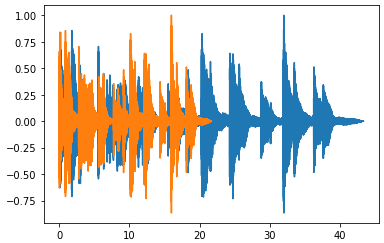
\includegraphics[scale=1]{fig/lab01/lab1_1.png}
		\caption{График фрагмента звука}
	\end{center}
\end{figure}

Далее узнаем спектр звука при помощи метода make\_spectrum и построим график для наглядности.
\begin{lstlisting}[language=Python]
spectrum = wave.make_spectrum()
spectrum.plot(high=5000)
\end{lstlisting}

\begin{figure}[H]
	\begin{center}
		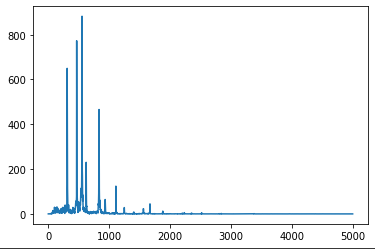
\includegraphics[scale=1]{fig/lab01/lab1_2.png}
		\caption{Спектр звука}
	\end{center}
\end{figure}

Мы видим, что данные расположились до 2Кгц, а график получился не информативный. Обрежем частоты выше 1250Гц, т.к. до них хранится вся важная информация - пики. На остальное смотреть не будем.

\begin{figure}[H]
	\begin{center}
		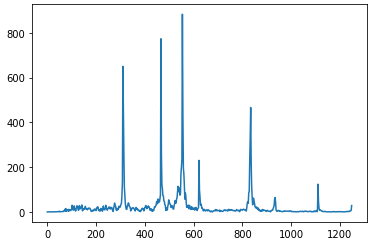
\includegraphics[scale=1]{fig/lab01/lab1_3.png}
		\caption{Спектр звука, частота меньше 1250 ГЦ}
	\end{center}
\end{figure}

Для точного понимания какие ноты сыграны выведем список пиков частот в спектре:

\begin{lstlisting}[language=Python]
spectrum.peaks()[:10]
\end{lstlisting}

\begin{lstlisting}
[(882.3500533686324, 554.0),
 (772.8812508117549, 466.0),
 (649.662314039115, 310.0),
 (466.0353893832775, 834.0),
 (455.88324114785496, 312.0),
 (435.6400663619303, 556.0),
 (328.0318016013845, 832.0),
 (260.99365239113706, 314.0),
 (251.02745102094198, 468.0),
 (234.35739758178494, 552.0)]
\end{lstlisting}


Находим соответствие музыкальных нот и частот из пиков:
\begin{itemize}
\item 554.36 Гц - С\# II
\item 466.16 Гц -  A\# I
\item 311.13 Гц - D\# I
\item 830.60 Гц - G\# II
\end{itemize}
Где \# обозначает "диез" или же черную ноту, римские цифра обозначают октаву ноты. У C\# II самая большая амплитуда, поэтому 554.36 Гц - доминирующая частота. Общая воспринимаемая высота звука зависит от основной частоты, тут она 311.13 Гц.

Добавим фильтр нижних частот. Все компоненты выше 540 ГЦ будут удалены. (На самом деле можно выбирать на сколько их ослаблять, но я решил на 100\%).

\begin{lstlisting}[language=Python]
spectrum2 = wave.make_spectrum()
spectrum2.low_pass(540)
spectrum2.plot(high=1000)
\end{lstlisting}

\begin{figure}[H]
	\begin{center}
		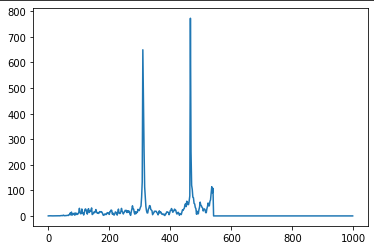
\includegraphics[scale=1]{fig/lab01/lab1_4.png}
		\caption{Спект с фильтром нижних частот}
	\end{center}
\end{figure}

Добавим фильтр верхних частот, и ослабим на половину компоненты до 500 Гц.

\begin{lstlisting}[language=Python]
spectrum2.high_pass(500,0.5)
spectrum2.plot(high=1000)
\end{lstlisting}

\begin{figure}[H]
	\begin{center}
		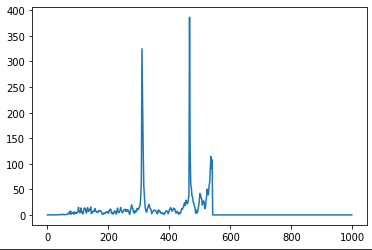
\includegraphics[scale=1]{fig/lab01/lab1_5.png}
		\caption{Спект с фильтром верхних частот}
	\end{center}
\end{figure}

Уберём частоты между Ре и Ля.

\begin{lstlisting}[language=Python]
spectrum2.band_stop(320,450)
spectrum2.plot(high=1000)
\end{lstlisting}



\begin{figure}[H]
	\begin{center}
		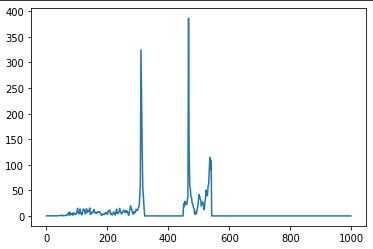
\includegraphics[scale=1]{fig/lab01/lab1_6.png}
		\caption{Получившийся спектр}
	\end{center}
\end{figure}

Звучание заметно изменилось из-за изменения доиминирующей частоты (её ампилитуда была уменьшена в 2 раза), но напоминает изначальный отрезок.

\begin{lstlisting}[language=Python]
wave = read_wave('1647_piano.wav')
wave = wave.segment(18.3,0.5)
spectrum2 = wave.make_spectrum()
spectrum2.high_pass(500)
spectrum2.plot(high=1000)
\end{lstlisting}

\begin{figure}[H]
	\begin{center}
		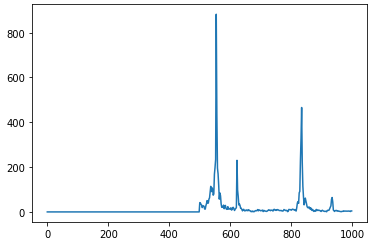
\includegraphics[scale=1]{fig/lab01/lab1_7.png}
		\caption{Отфильтрованные нижние компоненты}
	\end{center}
\end{figure}

Отфильтровав нижние частоты звук стал более высоким. Это логично, ведь ннизкие частоты придают более гулкое звучание, а на получившейся дорожке убраны все частоты, ниже 500.

\subsection{Упражнение 2}

Создайте сложный сигнал из объектов SinSignal и CosSignal, суммируя их. Обработайте сигнал для получения wave и прослушайте его. Вычислите Spectrum и распечатайте. Что произойдёт при добавлении частотных компонент, не кратных основным?


Берём два сигнала с частотой одной октавы. В итоге мы должны получить классическую синусоиду - волновой сигнал с очень высоким звучанием, однако из него при желании можно сделать бас, если опустить на несколько октав ниже.
\begin{lstlisting}[language=Python]
from thinkdsp import SinSignal, CosSignal
# https://nch-nch.ru/apps/frequency/
cos_sig1 = CosSignal(freq=784.00,amp=1,offset=0)
sin_sig2 = CosSignal(freq=392.00,amp=0.5,offset=0)
mix = cos_sig1 + sin_sig2
wave = mix.make_wave(duration=1)
wave.make_audio()
\end{lstlisting}

\begin{figure}[H]
	\begin{center}
		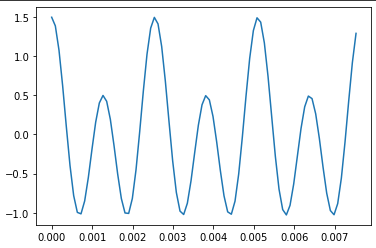
\includegraphics[scale=1]{fig/lab01/lab1_8.png}
		\caption{Суммированные сигналы}
	\end{center}
\end{figure}

\begin{lstlisting}[language=Python]
spectrum = wave.make_spectrum()
spectrum.plot(high = 1000)
\end{lstlisting}

\begin{figure}[H]
	\begin{center}
		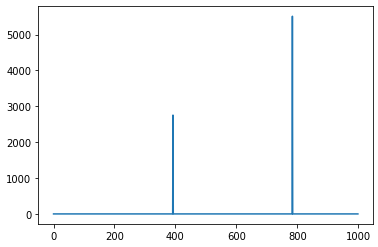
\includegraphics[scale=1]{fig/lab01/lab1_9.png}
		\caption{Спектр сигнала}
	\end{center}
\end{figure}

Добавим частоту из другой октавы. Должно получится ужасно для ушей.

\begin{lstlisting}[language=Python]
cos_signal3 = CosSignal(freq = 500, amp=0.25,offset = 0)
mix = mix + cos_signal3
wave = mix.make_wave(duration=1)
wave.make_audio()
\end{lstlisting}

На графике за 7мс не видно цикла.
\begin{figure}[H]
	\begin{center}
		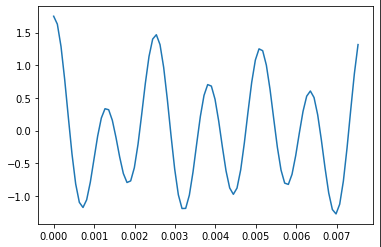
\includegraphics[scale=1]{fig/lab01/lab1_10.png}
		\caption{Получившийся сигнал}
	\end{center}
\end{figure}

Полученный звук не очень приятный.


\subsection{Упражнение 3}

Напишите функцию strech, берущую wave и коэффицент изменения. Она должна ускорять или замедлять сигнал изменением ts и framerate.

\noindent ts - моменты выборки сигнала, framerate - число выборок в единицу времени

\noindent если умножим ts на k - интервалы между моментами увеличатся в k раз

\noindent если framerate поделим на k - будет меньшее число подвыборок

\begin{lstlisting}[language=Python]
def stretch(wave, k):
  wave.ts *= k
  wave.framerate /= k
  return wave 
\end{lstlisting}


\subsection{Вывод}
В ходе первой ЛР я познакомился с основными понятиями при работе со звуками и сигналами в частности. Библиотека thinkDSP дает огромный потенциал для взаимодействия со звуками.
\newpage

\section{Гармоники}
\subsection{Упражнение 1}

Пилообразный сигнал линейно нарастает от -1 до 1, а затем резко падает до -1 и повторяется.

\noindent Напишите класс, называемый SawtoothSignal, расширяющий signal и предоставляющий evaluate для оценки пилообразного сигнала.

\noindent Вычислите спектр пилообразного сигнала. Как соотносится его гармоническая структура с тругольными с прямоугольными сигналами?

Для создания пилообразного сигнала создадим класс SawtoothSignal. В методе класса evaluate опишем число циклов и c помощью библиотеки numpy разделим число циклов. unbias - смещает сигнал а normalize масштабирует его до заданной амплитуды.

\begin{lstlisting}[language=Python]
import thinkdsp

class SawtoothSignal(thinkdsp.Sinusoid):
  def evaluate(self, ts):
    cycles = self.freq * ts + self.offset / np.pi / 2
    frac, _ = np.modf(cycles)
    ys = thinkdsp.normalize(thinkdsp.unbias(frac), self.amp)
    return ys
\end{lstlisting}

\noindent Далее отобразим график пилообразного сигнала.

\begin{lstlisting}[language=Python]
saw = SawtoothSignal()
saw.plot()
saw_wave = saw.make_wave(duration=3, framerate=10000)
\end{lstlisting}

\begin{figure}[H]
	\begin{center}
		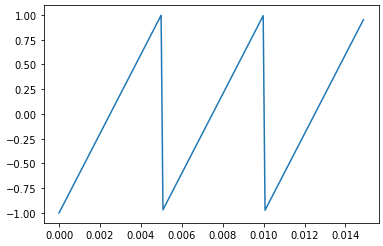
\includegraphics[scale=1]{fig/lab02/lab2_1.png}
		\caption{График пилообразного сигнала}
	\end{center}
\end{figure}

Мы действительно видим пилообразный сигнал. Далее сделаем экземпляр класса Wave для построения спектра сигнала.

\begin{lstlisting}[language=Python]
spectr = saw_wave.make_spectrum()
spectr.plot()
\end{lstlisting}

\begin{figure}[H]
	\begin{center}
		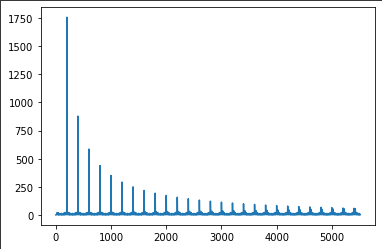
\includegraphics[scale=1]{fig/lab02/lab2_2.png}
		\caption{Спектр пилообразного сигнала}
	\end{center}
\end{figure}

Теперь сравним полученный спектр с треугольными и прямоугольными сигналами.

\begin{lstlisting}[language=Python]
triangle = TriangleSignal()
triangle.make_wave(duration=3, framerate=10000).make_spectrum().plot()
\end{lstlisting}

\begin{figure}[H]
	\begin{center}
		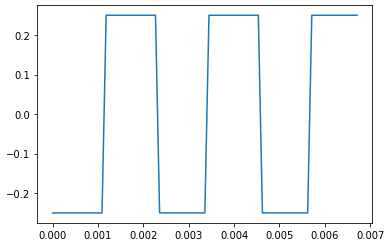
\includegraphics[scale=1]{fig/lab02/lab2_3.png}
		\caption{Спектр треугольного сигнала}
	\end{center}
\end{figure}

\begin{lstlisting}[language=Python]
square = SquareSignal()
square.make_wave(duration=3, framerate=10000).make_spectrum().plot()
\end{lstlisting}

\begin{figure}[H]
	\begin{center}
		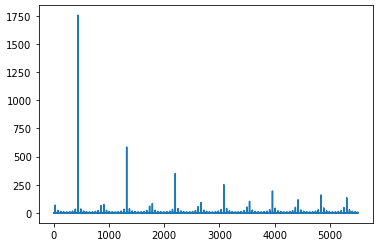
\includegraphics[scale=1]{fig/lab02/lab2_4.png}
		\caption{Спектр прямоугольного сигнала}
	\end{center}
\end{figure}

По сравнению с квадратным сигналом, пилообразный включает в себя четные и нечётные гармоники. Но оба сигнала снижают амплитуду обратно пропорциально частоте. По сравнению с изначальным сигналом, треугольный сигнал падает  1/f\^2 , а пилообразный  1/f .

\subsection{Упражнение 2}

Создайте прямугольный сигнал 1100 Гц и вычислите wave с выборками 10 000 кадров в секунду. Постройте спектр и убедитесь, что большинство гармоник "завёрнуты" из-за биений, слышно ли последствия этого при проигрывании?

\begin{lstlisting}[language=Python]
square = thinkdsp.SquareSignal(1100)
segment = square.make_wave(duration=1, framerate=10000)
spectr = segment.make_spectrum()
spectr.plot()
\end{lstlisting}

\begin{figure}[H]
	\begin{center}
		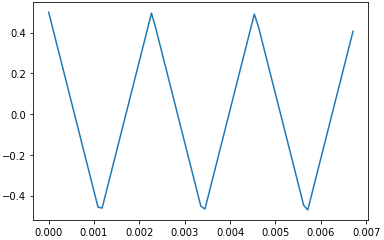
\includegraphics[scale=1]{fig/lab02/lab2_5.png}
		\caption{Спектр сигнала с биениями}
	\end{center}
\end{figure}

Из графика можно увидеть, что из-за фреймрейта, раввного 10.000 сигналы больших частот закольцовываются около 0Гц и 5Кгц - это называется биением. Когда мы слушаем получившийся звук - мы слышим основную частоту на 5КГц.


\subsection{Упражнение 3}

Возьмите объект спектра spectrum, и выведите первые несколько значений spectrum.fs, вы увидите, что частоты начинаются с нуля. Итак, «spectrum.hs[0]» — это величина компонента с частотой 0. Но что это значит?

\noindent Попробуйте этот эксперимент:

1. Сделать треугольный сигнал с частотой 440 и создать Волну длительностью 0,01 секунды. Постройте форму волны.

2. Создайте объект Spectrum и напечатайте spectrum.hs[0]. Каковы амплитуда и фаза этой составляющей?

3. Установите spectrum.hs[0] = 100. Создайте волну из модифицированного спектра и выведите ее. Как эта операция влияет на форму сигнала?

Создадим треугольный сигнал с частотой 440Hz и длительностью 0,01 сек, построим его график, распечатаем сигнал и распечатаем Spectrum.hs[0].


\begin{lstlisting}[language=Python]
signal = thinkdsp.TriangleSignal(440)
segment = signal.make_wave(0.01, framerate=10000)
segment.plot()
\end{lstlisting}

\begin{figure}[H]
	\begin{center}
		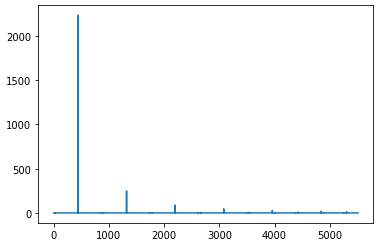
\includegraphics[scale=1]{fig/lab02/lab2_6.png}
		\caption{График сигнала}
	\end{center}
\end{figure}

Проверим что лежит в 0 элементе чисел спекторграммы.

\begin{lstlisting}[language=Python]
spectr = segment.make_spectrum()
spectr.hs[0]
\end{lstlisting}

\begin{lstlisting}
(1.375077994860476e-14+0j)
\end{lstlisting}
Видим комплексное число, с 0 мнимой частью. Сам элемент очень близок к нулю. Каждый элмент массива hs объекта Spectrum представялет собой комплексное число и соответствует частотоной компоненте: размах пропорционален амплитуде соответствующей компоненты, а угол - это фаза. Как видно из результатов выполнения кода, первый элемент массива hs - комплексное число, близкое к нулю, мнимая часть равна нулю.

\noindent Присвоим первый элемент 100 и посмотрим, что из этого выйдет.
\begin{lstlisting}[language=Python]
spectr.hs[0] = 100
spectr.make_wave().plot()
\end{lstlisting}

\begin{figure}[H]
	\begin{center}
		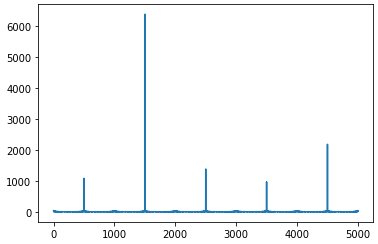
\includegraphics[scale=1]{fig/lab02/lab2_7.png}
		\caption{График сигнала с изменённым нулевым числом спекторграммы}
	\end{center}
\end{figure}

Как видно из полученного графика, сигнал сместился по вертикали. То есть первый элемент массив hs отвечает за смещение сигнали относительно вертикали. Если элемент близок или равен нулю, сигнал не смещенный.

\subsection{Упражнение 4}

Напишите функцию, которая принимает Spectrum в качестве параметра и модифицирует его, деля каждый элемент hs на соответствующую частоту из fs. Протестируйте свою функцию, используя один из файлов WAV в репозитории или любой объект Wave.

1. Рассчитайте спектр и начертите его.

2. Измените спектр, используя свою функцию, и снова начертите его.

3. Сделать волну из модифицированного Spectrum и прослушать ее. Как эта операция влияет на сигнал?


Исходя из последнего пункта первый элемент очень близок к нулю. Поэтому на него делить не надо, а то получим очень большие значения.

\begin{lstlisting}[language=Python]
def spec_div(spec):
  spec.hs[1:] /= spec.fs[1:]
  spec.hs[0] = 0
  spec.plot()

triangle = TriangleSignal()
wave = triangle.make_wave(duration=0.5, framerate=10000)
wave.make_audio()

spectr = wave.make_spectrum()
spectr.plot()
\end{lstlisting}

\begin{figure}[H]
	\begin{center}
		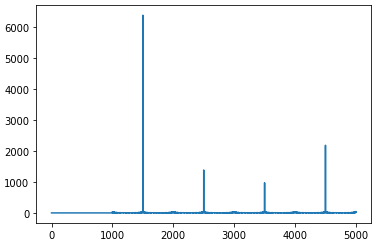
\includegraphics[scale=1]{fig/lab02/lab2_8.png}
		\caption{Спектр треугольного сигнала}
	\end{center}
\end{figure}

Применим написанную функцию.

\begin{lstlisting}[language=Python]
spec_div(spectr)
\end{lstlisting}

\begin{figure}[H]
	\begin{center}
		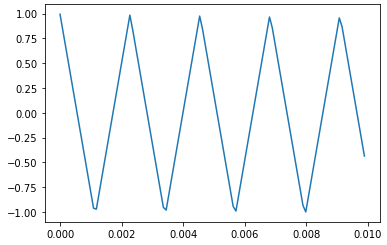
\includegraphics[scale=1]{fig/lab02/lab2_9.png}
		\caption{Спектр изменённого сигнала}
	\end{center}
\end{figure}

\begin{lstlisting}[language=Python]
spectr.make_wave().make_audio()
\end{lstlisting}

Видим. что ампилутуда очень поменялась, а частоты стоящие ближе к 0 Гц стали больше, чем следующие, что понятно.
Если сравнить полученные графики, можно сделать вывод, что функция действует как фильтр низких частот: частоты ослабляются на некоторую величину. Если сравнить две полученных звука на слух, то второй звучит более чисто, из-за отсутсвия низких часот, похож на звук синусоидального сигнала.

\subsection{Упражнение 5}

Треугольные и прямоугольные волны имеют только нечетные гармоники; пилообразная волна имеет как четные, так и нечетные гармоники. Гармоники прямоугольной и пилообразной волн затухают пропорционально $1/f$; гармоники треугольной волны затухают как $1/f^2$. Можете ли вы найти форму волны, в которой четные и нечетные гармоники затухают как $1/f^2$?

\noindent Подсказка: есть два способа подойти к этому: вы можете построить нужный сигнал путем сложения синусоид, или вы может начаться с сигнала, похожего на то, что вы хотите, и изменить его.


\noindent Не зря мы писали предыдущую функцию, поэтому возьмём пилообразный сигнал который имеет и четные и нечётные гармоники, а потом применим нашу функцию.

\begin{lstlisting}[language=Python]
saw_sign = SawtoothSignal(400)
saw_w = saw_sign.make_wave(duration=0.5, framerate=20000)
spectr = saw_w.make_spectrum()
spectr.plot()
decorate(xlabel='Frequency (Hz)')
\end{lstlisting}

\begin{figure}[H]
	\begin{center}
		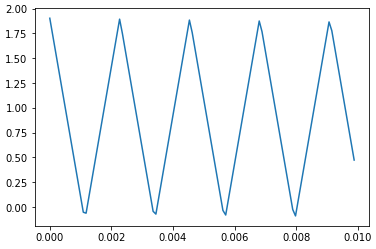
\includegraphics[scale=1]{fig/lab02/lab2_10.png}
		\caption{Спектр пилообразного сигнала}
	\end{center}
\end{figure}

Применим функцию для изменения амплитуды спада

\begin{lstlisting}[language=Python]
spec_div(spectr)
spectr.scale(400)
spectr.plot()
\end{lstlisting}

\begin{figure}[H]
	\begin{center}
		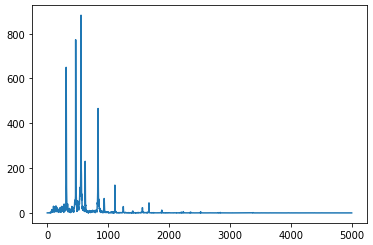
\includegraphics[scale=1]{fig/lab02/lab2_11.png}
		\caption{Спектр пилообразного сигнала после функции}
	\end{center}
\end{figure}

\begin{lstlisting}[language=Python]
spectr.make_wave().segment(duration=0.01).plot()
\end{lstlisting}

\begin{figure}[H]
	\begin{center}
		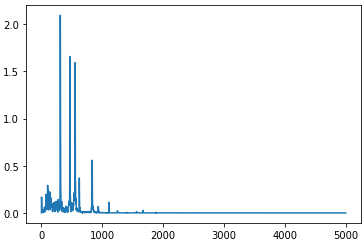
\includegraphics[scale=1]{fig/lab02/lab2_12.png}
		\caption{График сигнала}
	\end{center}
\end{figure}

Видно, что спектр спадает пропорционально квадрату частоты и при этом имеет четные и нечетные гармоники

\subsection{Вывод}

В ходе данной ладораторной работы были произведены различные действия с разными видами сигналов, а также были рассмотрены спектры и гармонические структуры и биения.
\newpage

\section{Непериодические сигналы}
\subsection{Упражнение 1}

Запустите и прослушайте примеры в файле chap03.ipynb. В примере с утечкой попробуйте заменить окно Хэмминга одним из других окон, предоставляемых NumPy, и посмотрите, как они влияют на утечку.

\begin{lstlisting}[language=Python]
signal = SinSignal(freq=440)
duration = signal.period * 30.25
wave = signal.make_wave(duration)
spectrum = wave.make_spectrum()
spectrum.plot(high=880)
\end{lstlisting}

\begin{figure}[H]
	\begin{center}
		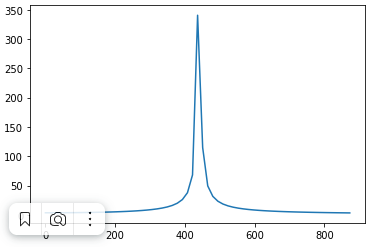
\includegraphics[scale=1]{fig/lab03/lab3_1.png}
		\caption{Рассматриваемый сигнал}
	\end{center}
\end{figure}

Посмотрим как выглядит спектограмма с использованием окна Хэмминга:

\begin{figure}[H]
	\begin{center}
		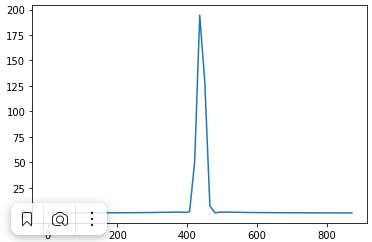
\includegraphics[scale=1]{fig/lab03/lab3_2.png}
		\caption{Сигнал с использованием окна Хэмминга}
	\end{center}
\end{figure}

Посмотрим остальные окна. Окно Бартлетта:
\begin{lstlisting}[language=Python]
wave = signal.make_wave(duration)
wave.ys *= np.bartlett(len(wave.ys))
spectrum = wave.make_spectrum()
spectrum.plot(high=880)
\end{lstlisting}
\begin{figure}[H]
	\begin{center}
		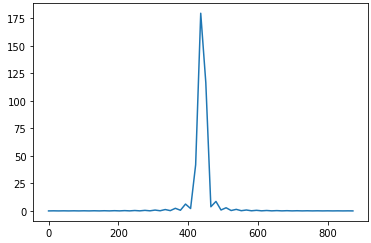
\includegraphics[scale=1]{fig/lab03/lab3_3.png}
		\caption{Сигнал с использованием окна Барлетта}
	\end{center}
\end{figure}
Можно заметить, что низкие амплитуды стали ломанными линиями.


Окно Блэкмена:
\begin{lstlisting}[language=Python]
wave = signal.make_wave(duration)
wave.ys *= np.blackman(len(wave.ys))
spectrum = wave.make_spectrum()
spectrum.plot(high=880)
\end{lstlisting}
\begin{figure}[H]
	\begin{center}
		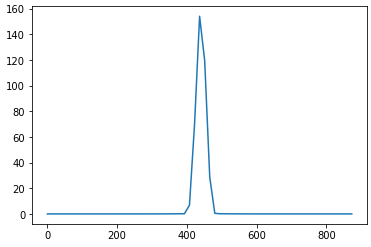
\includegraphics[scale=1]{fig/lab03/lab3_4.png}
		\caption{Сигнал с использованием окна Блэкмена}
	\end{center}
\end{figure}

Видим, что утечка стала линейно переходить к нужной частоте.

Окно Хэннинга:
\begin{lstlisting}[language=Python]
wave = signal.make_wave(duration)
wave.ys *= np.hanning(len(wave.ys))
spectrum = wave.make_spectrum()
spectrum.plot(high=880)
\end{lstlisting}
\begin{figure}[H]
	\begin{center}
		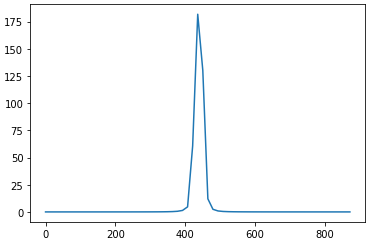
\includegraphics[scale=1]{fig/lab03/lab3_5.png}
		\caption{Сигнал с использованием окна Хэннинга}
	\end{center}
\end{figure}

Все оконные функции хорошо справились со своими задачами.
\subsection{Упражнение 2}


Напишите класс SawtoothChirp, расширяющий Chirp и переопределяющий evaluate для генерации пилообразного сигнала с линейно увеличивающейся частотой.

\noindent Нарисуйте эскиз спектограммы этого сигнала, затем распечатайте её. Эффект биение должен быть очевиден, а если сигнал внимательно прослушать, то биения можно и услышать.

\begin{lstlisting}[language=Python]
class SawtoothChirp(Chirp):

    def evaluate(self, ts):
        
        freqs = np.linspace(self.start, self.end, len(ts))
        dts = np.diff(ts, prepend=0)
        dphis = 2 * np.pi * freqs * dts
        phases = np.cumsum(dphis)
        cycles = phases / (2 * np.pi)
        frac, _ = np.modf(cycles)
        ys =  normalize(unbias(frac), self.amp)
        return ys
\end{lstlisting}

Для начала создадим звук:

\begin{lstlisting}[language=Python]
signal = SawtoothChirp(start = 440, end = 880)
wave = signal.make_wave(duration=1, framerate=4000)
wave.make_audio()
\end{lstlisting}

Слышно, как частота постепенно увеливается.

Выполним кратковременное преобразование Фурье и представим результат в виде спектограммы. По оси OY будет частота, по оси OX - время.

\begin{lstlisting}[language=Python]
sp = wave.make_spectrogram(256)
sp.plot()
\end{lstlisting}
\begin{figure}[H]
	\begin{center}
		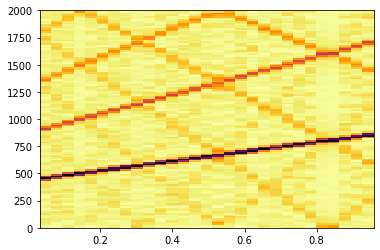
\includegraphics[scale=1]{fig/lab03/lab3_6.png}
		\caption{КПФ сигнала}
	\end{center}
\end{figure}

Черной линией обозначена наша основная частота, остальные частоты "отпрыгивают" от рамок координат и слышны на заднем плане.

\subsection{Упражнение 3}

Создайте пилообразный чирп, меняющийся от 2500 до 3000 Гц, и на его основе сгенерируйте сигнал длительностью 1 с и частотой кадоров 20 кГц. Нарисуйте, каким примерно будет Spectrum. Затем распечатайте Spectrum и посмотрите, правы ли вы.

\begin{lstlisting}[language=Python]
signal = SawtoothChirp(start=2500, end=3000)
wave = signal.make_wave(duration=1, framerate=20000)

wave.make_spectrum().plot()
\end{lstlisting}
\begin{figure}[H]
	\begin{center}
		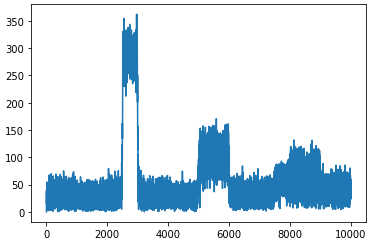
\includegraphics[scale=1]{fig/lab03/lab3_7.png}
		\caption{Спектр сигнала}
	\end{center}
\end{figure}

Видим, что гармоники накладываются друг на друга, и заметно что на частоте 2500 появляется возвышенность и на частоте около 5000 тоже. Это связано с тем, что в данном диапозоне равное изменение частоты занимает равное время.

\subsection{Упражнение 4}

В музыкальной терминологии «глиссандо» — это нота, которая скользит от одной высоты тона к другой, поэтому она похожа на чириканье. Найдите или сделайте запись глиссандо и постройте его спектрограмму.

Возьмём звук из репозитория учебника:

\begin{lstlisting}[language=Python]
if not os.path.exists('72475__rockwehrmann__glissup02.wav'):
    !wget https://github.com/AllenDowney/ThinkDSP/raw/master/code/72475__rockwehrmann__glissup02.wav
    

wave = read_wave('72475__rockwehrmann__glissup02.wav')

wave.make_spectrogram(512).plot(high=5000)
\end{lstlisting}
\begin{figure}[H]
	\begin{center}
		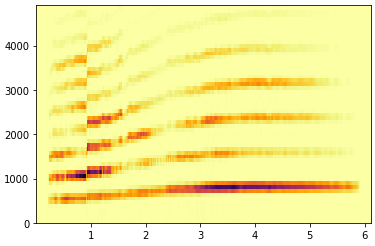
\includegraphics[scale=1]{fig/lab03/lab3_8.png}
		\caption{Спектрограмма сигнала}
	\end{center}
\end{figure}

Видим, что спектограмма очень похожа на наш чирп.

\subsection{Упражнение 5}

Тромбонист может играть глиссандо, выдвигая слайд тромбона и непрерывно дуя. По мере выдвижения ползуна общая длина трубки увеличивается, а результирующий шаг обратно пропорционален длине.
Предполагая, что игрок перемещает слайд с постоянной скоростью, как меняется ли частота со временем?

\noindent Напишите класс TromboneGliss, расширяющий класс Chirp и предоставляет evaluate. Создайте волну, имитирующую тромбон глиссандо от F3 вниз до C3 и обратно до F3. C3 — 262 Гц; F3 есть 349 Гц.
Напишем класс TromboneGliss расширяющий класс Chirp и переопределяющий метод evaluate

\begin{lstlisting}[language=Python]
class TromboneGliss(Chirp):

    
    def evaluate(self, ts):
        lengths = np.linspace(1.0 / self.start, 1.0 / self.end, len(ts))
        freqs = 1 / lengths
        dts = np.diff(ts, prepend=0)
        dphis = np.pi * 2 * freqs * dts
        phases = np.cumsum(dphis)
        ys = self.amp * np.cos(phases)
        return ys
\end{lstlisting}

Соединим сигналы:
\begin{lstlisting}[language=Python]
signal1 = TromboneGliss(262, 349)
wave1 = signal.make_wave(duration=1)

signal2 = TromboneGliss(349, 262)
wave2 = signal2.make_wave(duration=1)

result = wave1 | wave2
sp = result.make_spectrogram(1024)
sp.plot(high=1000)
\end{lstlisting}
\begin{figure}[H]
	\begin{center}
		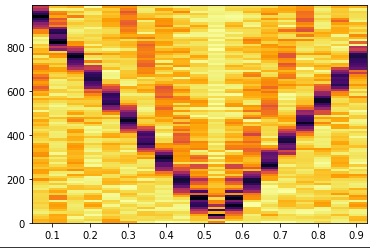
\includegraphics[scale=1]{fig/lab03/lab3_9.png}
		\caption{Спектрограмма сигнала}
	\end{center}
\end{figure}

Отчётливо слышно, как друг за другом идут 2 части.


\subsection{Упражнение 6}

Сделайте или найдите запись серии гласных звуков и посмотрите на спектрограмму. Сможете ли вы различить разные гласные?

Снова воспользуемся репозиторием учебника и возьмем оттуда звуки гласных:

\begin{lstlisting}[language=Python]
if not os.path.exists('87778__marcgascon7__vocals.wav'):
    !wget https://github.com/AllenDowney/ThinkDSP/raw/master/code/87778__marcgascon7__vocals.wav
wave = read_wave('87778__marcgascon7__vocals.wav')
wave.make_spectrogram(1024).plot(1000)
\end{lstlisting}
\begin{figure}[H]
	\begin{center}
		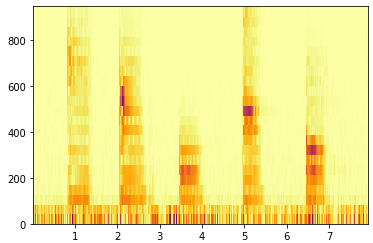
\includegraphics[scale=1]{fig/lab03/lab3_10.png}
		\caption{Спектрограмма гласных звуков}
	\end{center}
\end{figure}

На спектограмме видны пики, они и будут нашими гласными.

\subsection{Вывод}

В ходе данной ЛР были рассмотрены сигналы, частотные компоненты которых изменяются со временем. Такие сигналы называются апериодическими. Кроме того были рассмотрены спектрограммы - способ визуализации вышеприведенных сигналов.
\newpage

\section{Шумы}
\subsection{Упражнение 1}

«A Soft Murmur» — это веб-сайт, на котором можно послушать множество естественных источников шума, включая дождь, волны, ветер и т. д. 

\noindent На http://asoftmurmur.com/about/ вы можете найти их список записей, большинство из которых находится на http://freesound.org.

\noindent Загрузите несколько таких файлов и вычислите спектр каждого сигнала. Спектр мощности похож на белый шум, розовый шум, или броуновский шум? Как изменяется спектр во времени?

Возьмем звук моря и выделим два сегмента.

\begin{lstlisting}[language=Python]
if not os.path.exists('13793__soarer__north-sea.wav'):
    !wget https://drive.google.com/file/d/1OJcFGqEs128g5T8pQmgaERBHX8cyFSsT/view?usp=sharing
from thinkdsp import read_wave
wave = read_wave('13793__soarer__north-sea.wav')
wave.make_audio()
segment = wave.segment(start=15, duration=1.0)
segment.make_audio()
segment.plot()
\end{lstlisting}
\begin{figure}[H]
	\begin{center}
		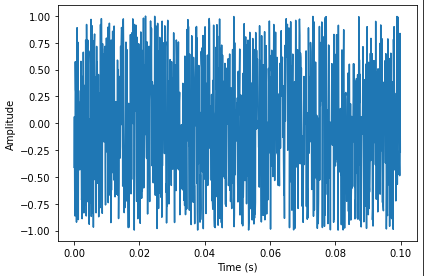
\includegraphics[scale=1]{fig/lab04/lab4_1.png}
		\caption{График сигнала}
	\end{center}
\end{figure}

Определим характеристики шума.

\begin{lstlisting}[language=Python]
from thinkdsp import decorate
spectrum.plot_power()

loglog = dict(xscale='log', yscale='log')
decorate(xlabel='Frequency (Hz)',
         ylabel='Power', 
         **loglog)
\end{lstlisting}
\begin{figure}[H]
	\begin{center}
		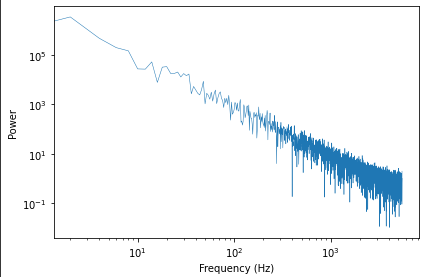
\includegraphics[scale=1]{fig/lab04/lab4_2.png}
		\caption{Спектр в логорифмическом масштабе}
	\end{center}
\end{figure}

График напоминает белый шум. Далее возьмем идущий за ним другой сегмент.

\begin{lstlisting}[language=Python]
segmentNext = wave.segment(start=16, duration=1.0)
segmentNext.make_audio()

spectrumNext = segmentNext.make_spectrum()
spectrum.plot_power()
spectrumNext.plot_power()

loglog = dict(xscale='log', yscale='log')
decorate(xlabel='Frequency (Hz)',
         ylabel='Power', 
         **loglog)
\end{lstlisting}
\begin{figure}[H]
	\begin{center}
		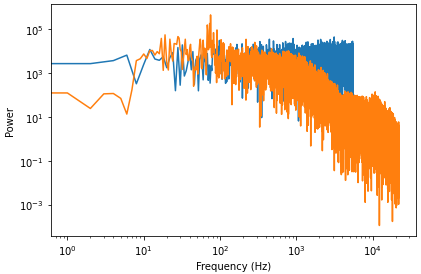
\includegraphics[scale=1]{fig/lab04/lab4_3.png}
		\caption{Сравнение спектров в логорифмическом масштабе}
	\end{center}
\end{figure}


\subsection{Упражнение 2}

Реализуйте метод Бартлетта\cite{barlett} и используйте его для оценки спектра мощности шумового сигнала. Подсказка: посмотрите на реализацую make\_spectrogram.

Реализуем метод Бартлетта для оценки спектра мощности шумового сигнала. Данный метод будет разделять сигнал на сегменты, вычислять для них разложение Фурье, вычислять сумму квадратов, находить среднее и вычислять корень.


\begin{lstlisting}[language=Python]
from thinkdsp import Spectrum

def make_barlett(wave, N, flag=True):
  spectrogram = wave.make_spectrogram(N,flag)
  spec_mac = spectrogram.spec_map.values()

  powers = []
  for spectrum in spec_mac:
    powers.append(spectrum.power)
  
  hs = np.sqrt(sum(powers)/ len(powers))
  fs = next(iter(spec_mac)).fs

  return Spectrum(hs, fs, wave.framerate)
\end{lstlisting}

Проведем тестирование на сигнале с предыдущего задания.

\begin{lstlisting}[language=Python]
barlett = make_barlett(segmentNext,1024)
barlett.plot_power()
decorate(xlabel='Frequency (Hz)', 
         ylabel='Power', 
         **loglog)
\end{lstlisting}

\begin{figure}[H]
	\begin{center}
		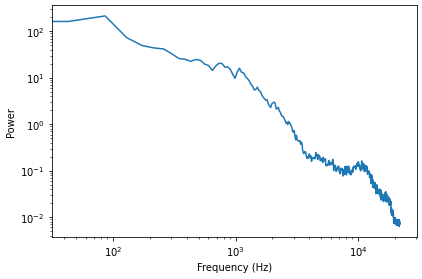
\includegraphics[scale=1]{fig/lab04/lab4_4.png}
		\caption{Результат работы функции}
	\end{center}
\end{figure}


\subsection{Упражнение 3}

Загрузите в виде CSV-файла исторические данные о ежедневной цене BitCoin. Откройте этот файл и вычислите спектр цен BitCoin как функцию времени. Похоже ли это на белый, розовый или броуновский шум?

Скачаем csv файл с ценами на биткоин.

\begin{lstlisting}[language=Python]
if not os.path.exists('market-price.csv'):
    !wget https://github.com/pimenov01/telecom/raw/main/files/market-price.csv
import csv
worth = []
with open('market-price.csv') as File:
  reader = csv.reader(File, delimiter=',', quotechar=',',
                        quoting=csv.QUOTE_MINIMAL)
  for row in reader:
    worth.append(row[1])
worth = worth [1:]
days = a=np.arange(0,len(worth))
\end{lstlisting}
\begin{lstlisting}[language=Python]
from thinkdsp import Wave
wave = Wave(worth,days,1)
spectrum = wave.make_spectrum()
spectrum.plot_power()
decorate(xlabel='Частота',
         ylabel='Мощность', 
         **loglog)
\end{lstlisting}

\begin{figure}[H]
	\begin{center}
		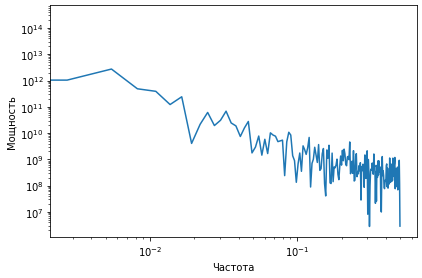
\includegraphics[scale=1]{fig/lab04/lab4_5.png}
		\caption{Спектрограмма цен BitCoin в логорифмическом формате}
	\end{center}
\end{figure}

Больше всего напоминает красный шум.

\subsection{Упражнение 4}

Счетчик Гейгера — это прибор, который регистрирует радиацию. Когда ионизирующая частица попадает на детектор, он генерирует всплеск тока. Общий вывод в определенный момент времени можно смоделировать как некоррелированный шум Пуассона (UP), где каждая выборка представляет собой случайную величину из распределения Пуассона, которая соответствует количеству частиц, обнаруженных в течение интервала.

Напишите класс с именем `UncorrelatedPoissonNoise`, который наследуется от `\_Noise` и предоставляет `evaluate`. Он должен использовать `np.random.poisson` для генерации случайных значений из распределения Пуассона. Параметр этой функции, lam, представляет собой среднее число частиц в течение каждого интервала. Вы можете использовать атрибут `amp`, чтобы указать `lam`. Например, если частота кадров равна 10 кГц, а amp равно 0,001, мы ожидаем около 10 «кликов» в секунду.

Создайте около секунды шума UP и послушайте его. Для низких значений «ампер», например 0,001, это должно звучать как счетчик Гейгера. Для более высоких значений это должно звучать как белый шум. Вычислите и начертите спектр мощности, чтобы увидеть, похож ли он на белый шум.

Напишем класс UncorrelatedPoissonNoise, который наследуется от класса thinkdsp\_Noise и который моделирует некоррелированный пуассонвский шум (UP).

\begin{lstlisting}[language=Python]
from thinkdsp import *
class UncorrelatedPoissonNoise(Noise):
    def evaluate(self, ts):
        ys = np.random.poisson(self.amp, len(ts))
        return ys
\end{lstlisting}
Сгенирируем сигнал с маленькой амплитудой, звук должен быть похож на счетчик Гейгера.
\begin{lstlisting}[language=Python]
firstSignal = UncorrelatedPoissonNoise(amp=0.001)
firstWave = firstSignal.make_wave(duration=1, framerate=10000)
firstWave.make_audio()
\end{lstlisting}

Далее сгенерируем сигнал с большой амплитудой.

\begin{lstlisting}[language=Python]
secondSignal = UncorrelatedPoissonNoise(1)
secondWave = secondSignal.make_wave(duration=1,framerate = 10000)
secondWave.make_audio()
\end{lstlisting}

Посмотрим на характеристики данных сигналов:

\begin{lstlisting}[language=Python]
spectrum1 = firstWave.make_spectrum()
spectrum2 = secondWave.make_spectrum()

spectrum1.plot_power()
spectrum2.plot_power()

decorate(xlabel='Частота', 
         ylabel='Мощность', 
         **loglog)
\end{lstlisting}
\begin{figure}[H]
	\begin{center}
		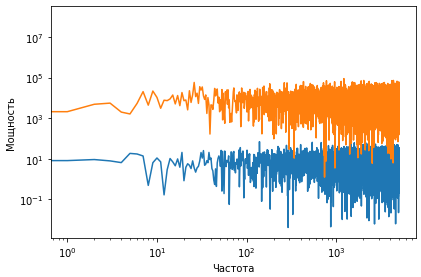
\includegraphics[scale=1]{fig/lab04/lab4_6.png}
		\caption{Сравнение спектров}
	\end{center}
\end{figure}

Видно, что при увеличении амплитуды звук больше похож на белый шум.

\subsection{Упражнение 5}

В этой главе описан алгоритм генерации розового шума. Концептуально простой, но вычислительно затратный. Есть более эффективные альтернативы, такие как алгоритм Восса-Маккартни.

Используем алгоритм Voss-McCartney для генерации розового шума.

\begin{lstlisting}[language=Python]
def voss(nrows, ncols=16):
    array = np.empty((nrows, ncols))
    array.fill(np.nan)
    array[0, :] = np.random.random(ncols)
    array[:, 0] = np.random.random(nrows)
    
    n = nrows
    cols = np.random.geometric(0.5, n)
    cols[cols >= ncols] = 0
    rows = np.random.randint(nrows, size=n)
    array[rows, cols] = np.random.random(n)

    df = pd.DataFrame(array)
    df.fillna(method='ffill', axis=0, inplace=True)
    total = df.sum(axis=1)

    return total.values
\end{lstlisting}

\begin{lstlisting}[language=Python]
ys = voss(11025,16)
wave = Wave(ys)
wave.plot()
\end{lstlisting}

\begin{figure}[H]
	\begin{center}
		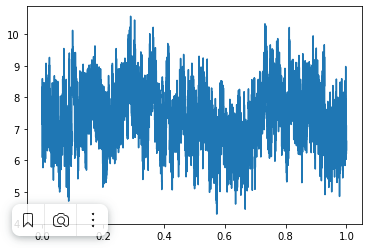
\includegraphics[scale=1]{fig/lab04/lab4_7.png}
		\caption{Сгенерированный сигнал}
	\end{center}
\end{figure}

\begin{lstlisting}[language=Python]
spectrum = wave.make_spectrum()
spectrum.hs[0] = 0
spectrum.plot_power()
decorate(xlabel='Частота',
         ylabel='Мощность',
         **loglog)
\end{lstlisting}
\begin{figure}[H]
	\begin{center}
		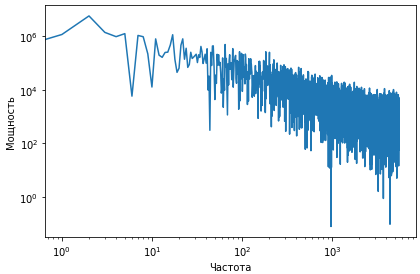
\includegraphics[scale=1]{fig/lab04/lab4_8.png}
		\caption{Спектр сигнала}
	\end{center}
\end{figure}

\begin{lstlisting}[language=Python]
spectrum.estimate_slope()[0]
\end{lstlisting}

-0.9809177359665783

\noindent Видим, что в итоге был получен сигнал розового шума.

\subsection{Вывод}

В ходе данной ЛР были изучены различные виды шумов: белый, розовый, красный и т. д. Шум - это сишнал, представленный компонентами с разными частотами, но не имеющий гармонической структура периодических сигналов.

\newpage

\section{Автокорреляция }
\subsection{Упражнение 1}

Оцените высоты тона вокального чирпа для нескольких времён начала сегмента.

\begin{lstlisting}[language=Python]
if not os.path.exists('28042__bcjordan__voicedownbew.wav'):
    !wget https://github.com/AllenDowney/ThinkDSP/raw/master/code
    /28042__bcjordan__voicedownbew.wav
from thinkdsp import read_wave
wave = read_wave('28042__bcjordan__voicedownbew.wav')
wave.normalize()
wave.make_audio()

duration = 0.01
segment1 = wave.segment(start=0.5, duration=duration)
segment1.plot()
segment2 = wave.segment(start=0.6, duration=duration)
segment2.plot()
segment3 = wave.segment(start=0.7, duration=duration)
segment3.plot()
\end{lstlisting}
\begin{figure}[H]
	\begin{center}
		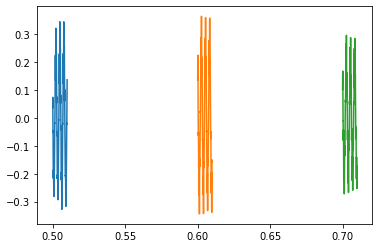
\includegraphics[scale=1]{fig/lab05/lab5_1.png}
		\caption{График сегментов}
	\end{center}
\end{figure}

Используем автокореляцию.

\begin{lstlisting}[language=Python]
lags1, corrs1 = autocorr(segment1)
plt.plot(lags1, corrs1, color='black')
decorate(xlabel='Lag', ylabel='Correlation', ylim=[-1, 1])

lags2, corrs2 = autocorr(segment2)
plt.plot(lags2, corrs2)
decorate(xlabel='Lag', ylabel='Correlation', ylim=[-1, 1])

lags3, corrs3 = autocorr(segment3)
plt.plot(lags3, corrs3, color='red')
decorate(xlabel='Lag', ylabel='Correlation', ylim=[-1, 1])
\end{lstlisting}
\begin{figure}[H]
	\begin{center}
		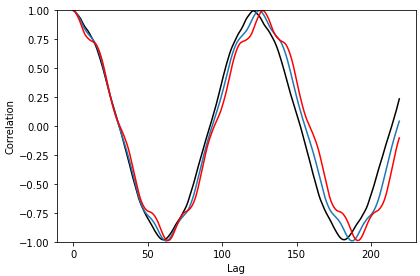
\includegraphics[scale=1]{fig/lab05/lab5_2.png}
		\caption{Автокорреляция сигналов}
	\end{center}
\end{figure}

Вычислим lag

\begin{lstlisting}[language=Python]
low = 50
high = 200
lag1 = np.array(corrs1[low:high]).argmax() + low
lag2 = np.array(corrs2[low:high]).argmax() + low
lag3 = np.array(corrs3[low:high]).argmax() + low

lag1,lag2, lag3
\end{lstlisting}
\begin{lstlisting}
(121, 125, 127)
\end{lstlisting}

Вычислим периоды

\begin{lstlisting}[language=Python]
period1 = lag1 / segment1.framerate
period2 = lag2 / segment2.framerate
period3 = lag3 / segment3.framerate
period1, period2, period3
\end{lstlisting}
\begin{lstlisting}
(0.0027437641723356007, 0.002834467120181406, 0.0028798185941043084)
\end{lstlisting}

Соответствующие периодам частоты:

\begin{lstlisting}[language=Python]
frequency1 = 1 / period1
frequency2 = 1 / period2
frequency3 = 1 / period3
frequency1, frequency2, frequency3
\end{lstlisting}
\begin{lstlisting}
(364.4628099173554, 352.8, 347.244094488189)
\end{lstlisting}

\subsection{Упражнение 2}
Инкапсулировать код автокорреляции для оценки основной частоты периодического сигнала в функцию, названную estimate\_fundamental, и исользуйте её для отслеживания высоты тона записанного звука.

Для тестирования возьмем звук из прошлого номера.

\begin{lstlisting}[language=Python]
wave.make_spectrogram(2048).plot(high=4000)
\end{lstlisting}
\begin{figure}[H]
	\begin{center}
		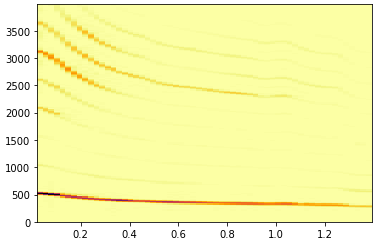
\includegraphics[scale=1]{fig/lab05/lab5_3.png}
		\caption{Спектрограмма звука}
	\end{center}
\end{figure}

Объединим весь код из предыдущего пункта в одну функцию.

\begin{lstlisting}[language=Python]
def estimate_fundamental(segment, low=50, high=200):
  lags, corrs = autocorr(segment)
  lag = np.array(corrs[low:high]).argmax() + low
  period = lag / segment.framerate
  frequency = 1 / period
  return frequency
\end{lstlisting}

\begin{lstlisting}[language=Python]
estimate_fundamental(segment1)
\end{lstlisting}
\begin{lstlisting}
364.4628099173554
\end{lstlisting}

Сделаем оценку высоты тона, применяя разделение на сегменты.

\begin{lstlisting}[language=Python]
duration = wave.duration
step = 0.02
start = 0
time = []
frequencys = []
while start + step < duration:
  time.append(start + step/2)
  frequencys.append(estimate_fundamental(wave.segment(start=start,duration=step)))
  start += step
wave.make_spectrogram(2048).plot(high=900)
plt.plot(time, frequencys, color='black')
decorate(xlabel='Time (s)', ylabel='Frequency (Hz)')
\end{lstlisting}
\begin{figure}[H]
	\begin{center}
		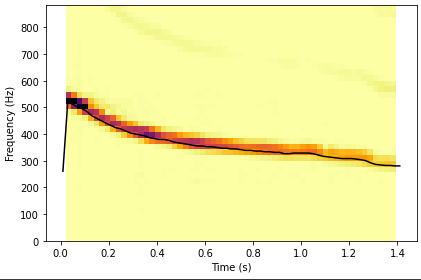
\includegraphics[scale=1]{fig/lab05/lab5_4.png}
		\caption{Результат оценки}
	\end{center}
\end{figure}

\subsection{Упражнение 3}

Вычислить автокорреляцию цен в платёжной системе Bitcoin. Оценить автокореляцию и проверить на признаки переодичности процесса.

\begin{lstlisting}[language=Python]
if not os.path.exists('market-pric.csv'):
    if not os.path.exists('market-pric.csv'):
    !wget https://github.com/pimenov01/telecom/raw/main/files/data.csv

import pandas as pd
from thinkdsp import Wave

df = pd.read_csv('market-pric.csv', parse_dates=[0])
ys = df['market-price']
ts = df.index

w = Wave(ys, framerate=1)
w.plot()

\end{lstlisting}
\begin{figure}[H]
	\begin{center}
		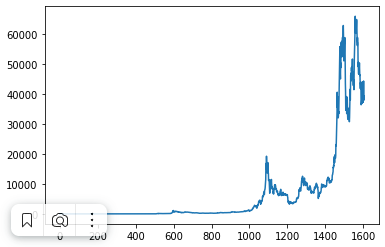
\includegraphics[scale=1]{fig/lab05/lab5_5.png}
		\caption{График цены на BitCoin}
	\end{center}
\end{figure}

Вычислим автокорреляцию:

\begin{lstlisting}[language=Python]
lags, corrs = autocorr(w)
plt.plot(lags, corrs)
decorate(xlabel='Lag',
        ylabel='Correlation')
\end{lstlisting}
\begin{figure}[H]
	\begin{center}
		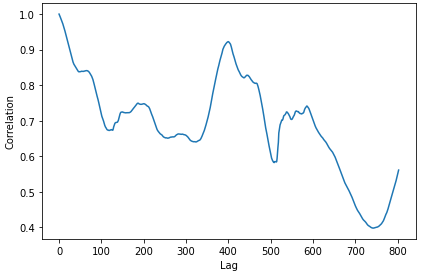
\includegraphics[scale=1]{fig/lab05/lab5_6.png}
		\caption{Автокорреляция функции цены на BitCoin}
	\end{center}
\end{figure}

По графику видно, что есть резкие спады и повышения. Процесс может напоминать переодичность.

\subsection{Упражнение 4}

В репозитории этой книги есть блокнот Jupyter под названием saxophone.ipynb, в котором исследуются автокорреляция, восприятие высоты тона и явление, называемое подавленная основная. Прочтите этот блокнот и «погоняйте» примеры. Выберите другой сегмент записи и вновь поработайте с примерами.

\begin{lstlisting}[language=Python]
if not os.path.exists('100475__iluppai__saxophone-weep.wav'):
    !wget https://github.com/AllenDowney/ThinkDSP/raw/master/code/100475__iluppai__saxophone-weep.wav
wave = read_wave('100475__iluppai__saxophone-weep.wav')
wave.normalize()
wave.make_audio()
spectrogram = wave.make_spectrogram(seg_length=1024)
spectrogram.plot(high=3000)
decorate(xlabel='Time (s)', ylabel='Frequency (Hz)')
\end{lstlisting}
\begin{figure}[H]
	\begin{center}
		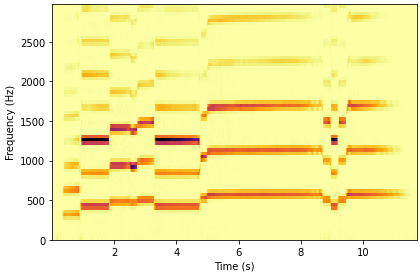
\includegraphics[scale=1]{fig/lab05/lab5_7.png}
		\caption{Спектрограмма сегмента}
	\end{center}
\end{figure}

Используем функции из блокнтота из репозитория и используем их для другого сегмента.

\begin{lstlisting}[language=Python]
segment = wave.segment(start=4.0, duration=0.2)
segment.make_audio()
spectrum = segment.make_spectrum()
spectrum.plot(high=5000)
decorate(xlabel='Frequency', ylabel='Amplitude')
\end{lstlisting}

\begin{figure}[H]
	\begin{center}
		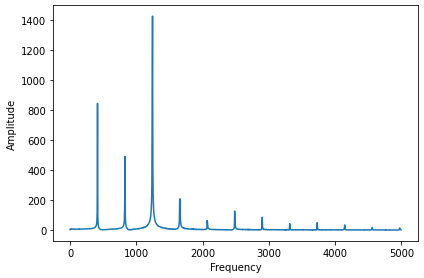
\includegraphics[scale=1]{fig/lab05/lab5_8.png}
		\caption{Спектр другого сегмента}
	\end{center}
\end{figure}

Пики в спектре находятся на 1245, 415 и 830 Гц.

\begin{lstlisting}[language=Python]
spectrum.peaks()[:10]
\end{lstlisting}

\begin{lstlisting}
[(1425.371205417228, 1245.0),
 (844.1565084866448, 415.0),
 (810.3146734198679, 1240.0),
 (491.1468807713408, 830.0),
 (395.0157320768441, 1250.0),
 (285.5428668623747, 1235.0),
 (220.80813321938248, 1255.0),
 (208.75420107735613, 1660.0),
 (205.643155157793, 1655.0),
 (180.59606616391875, 1230.0)]
\end{lstlisting}

Сравним наш сегмент с треугольным сигналом.

\begin{lstlisting}[language=Python]
from thinkdsp import TriangleSignal
TriangleSignal(freq=415).make_wave(duration=0.2).make_audio()
segment.make_audio()
\end{lstlisting}

У сигналов одинаковая воспринимаемая частота звука. Для понимания процесса восприятия основной частоты испольщуем АКФ.

\begin{lstlisting}[language=Python]
def autocorr2(segment):
    corrs = np.correlate(segment.ys, segment.ys, mode='same')
    N = len(corrs)
    lengths = range(N, N//2, -1)

    half = corrs[N//2:].copy()
    half /= lengths
    half /= half[0]
    return half

corrs = autocorr2(segment)
plt.plot(corrs[:500])
\end{lstlisting}

\begin{figure}[H]
	\begin{center}
		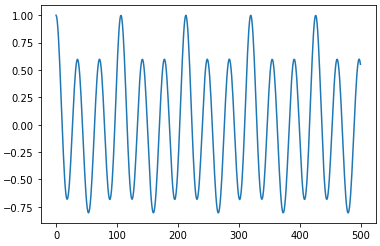
\includegraphics[scale=1]{fig/lab05/lab5_9.png}
		\caption{График после АКФ}
	\end{center}
\end{figure}

Первый пик находился возле lag 100.

Найдём основную частоту при помощи написанной ранее функции.

\begin{lstlisting}[language=Python]
estimate_fundamental(segment)
\end{lstlisting}

\begin{lstlisting}
416.0377358490566
\end{lstlisting}

Воспринимаемая высота тона не изменится, если мы полностью удалим основной тон. Вот как выглядит спектр, если мы используем фильтр верхних частот, чтобы стереть основные частоты.

\begin{lstlisting}[language=Python]
spectrum2 = segment.make_spectrum()
spectrum2.high_pass(600)
spectrum2.plot(high=3000)
decorate(xlabel='Frequency (Hz)', ylabel='Amplitude')
\end{lstlisting}

\begin{figure}[H]
	\begin{center}
		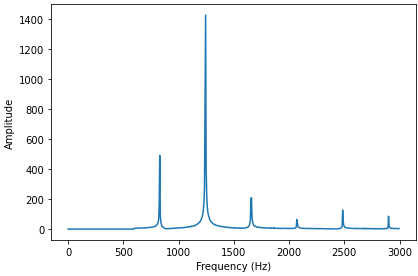
\includegraphics[scale=1]{fig/lab05/lab5_10.png}
		\caption{Спектр после ФНЧ}
	\end{center}
\end{figure}

Это явление называется "отсутствующим фундаментом"
Чтобы понять, почему мы слышим частоту, которой нет в сигнале, полезно взглянуть на функцию автокорреляции (ACF).

\begin{lstlisting}[language=Python]
corrs = autocorr2(segment2)
plt.plot(corrs[:500])
\end{lstlisting}

\begin{figure}[H]
	\begin{center}
		\includegraphics[scale=1]{fig/lab05/lab5_11.png}
		\caption{Полученный график}
	\end{center}
\end{figure}

\begin{lstlisting}[language=Python]
estimate_fundamental(segment)
\end{lstlisting}

\begin{lstlisting}
416.0377358490566
\end{lstlisting}

Таким образом, результаты работы показывают, что восприятие высоты тона основано не только на спектральном анализе, но и на чем-то вроде автокорреляции.

\subsection{Вывод}

В ходе данной ЛР мы изучали корреляцию и ее влияние на сигналы. Также был написан код для сигнала с "отсутствующим фундаментом".



\newpage

\section{Дискретное косинусное преобразование }
\subsection{Упражнение 1}

Показать на графике время работы analyze1 и analyze2 в логарифмическом масштабе. Сравнить с scipy.fftpack.dct.

\begin{lstlisting}[language=Python]
def analyze1(ys, fs, ts):
    args = np.outer(ts, fs)
    M = np.cos(PI2 * args)
    amps = np.linalg.solve(M, ys)
    return amps
def analyze2(ys, fs, ts):
    args = np.outer(ts, fs)
    M = np.cos(PI2 * args)
    amps = M.dot(ys) / 2
    return amps
\end{lstlisting}

Зазадим размер массива степенями двойки.

\begin{lstlisting}[language=Python]
ns = 2 ** np.arange(5,10)
\end{lstlisting}

\begin{lstlisting}[language=Python]
best_analyze1 = []
for n in ns:
    ts = (0.5 + np.arange(n)) / n
    freqs = (0.5 + np.arange(n)) / 2
    ys = wave.ys[:n]
    best =  %timeit -r1 -o analyze1(ys,freqs,ts)
    best_analyze1.append(best.best)
best_analyze2 = []
for n in ns:
    ts = (0.5 + np.arange(n)) / n
    freqs = (0.5 + np.arange(n)) / 2
    ys = wave.ys[:n]
    best =  %timeit -r1 -o analyze2(ys,freqs,ts)
    best_analyze2.append(best.best)
best_dct = []
for n in ns:
    ys = wave.ys[:n]
    best =  %timeit -r1 -o scipy.fftpack.dct(ys, type=3)
    best_dct.append(best.best)
plt.plot(ns, best_analyze1, label='analyze1')
plt.plot(ns, best_analyze2, label='analyze2')
plt.plot(ns, best_dct, label='fftpack.dct')
loglog = dict(xscale='log', yscale='log')
decorate(xlabel='Wave length (N)', ylabel='Time (s)', **loglog)
\end{lstlisting}

\begin{figure}[H]
	\begin{center}
		\includegraphics[scale=1]{fig/lab06/lab6_1.png}
		\caption{Время работы различных методов ДКП}
	\end{center}
\end{figure}

Не смотря на теоритическое время исполнения, время analyze1 получилсось пропорциональным  n2 .

\subsection{Упражнение 2}

Реализовать алгоритм сжатия для музыки или речи.

Выберем звук для сжатия:
\begin{lstlisting}[language=Python]
if not os.path.exists('1647_piano.wav'):
    !wget https://github.com/pimenov01/telecom/raw/main/files/1647_piano.wav
    wave = read_wave('1647_piano.wav')
\end{lstlisting}

Для начала возьмём небольшой сегмент:

\begin{lstlisting}[language=Python]
segment = wave.segment(start = 1.7,duration = 1.0)
segment.normalize()
segment.make_audio()
\end{lstlisting}

Используем DCT вместо DFT.

\begin{lstlisting}[language=Python]
dct = segment.make_dct()
dct.plot(high = 5000)
\end{lstlisting}
\begin{figure}[H]
	\begin{center}
		\includegraphics[scale=1]{fig/lab06/lab6_2.png}
		\caption{Спектр сигнала полученный при помощи ДКП}
	\end{center}
\end{figure}

\begin{lstlisting}[language=Python]
def filtering(dct,limit = 0):
  for i, amp in enumerate(dct.amps):
    if np.abs(amp) < limit:
      dct.hs[i] = 0
\end{lstlisting}

\begin{lstlisting}[language=Python]
filtering(dct,1000)
dct.plot(high = 5000)
\end{lstlisting}
\begin{figure}[H]
	\begin{center}
		\includegraphics[scale=1]{fig/lab06/lab6_3.png}
		\caption{ДКП после фильтрации}
	\end{center}
\end{figure}

Теперь подберём значение, чтобы результат звучал как исходник. Для эффективного хранения данных можно использовать разряженные массивы.

\subsection{Управжнение 3}

В блокноте phase.ipynb взять другой сегмент звука и повторить эксперименты.

\begin{lstlisting}[language=Python]
signal = SawtoothSignal(freq=500, offset=0)
wave = signal.make_wave(duration=0.5, framerate=40000)
wave.segment(start=0.005,duration=0.01).plot()
decorate(xlabel='Time (s)')
\end{lstlisting}
\begin{figure}[H]
	\begin{center}
		\includegraphics[scale=1]{fig/lab06/lab6_4.png}
		\caption{Выбранный сегмент}
	\end{center}
\end{figure}

\begin{lstlisting}[language=Python]
spectrum = wave.make_spectrum()
spectrum.plot()
decorate(xlabel='Frequency (Hz)',
         ylabel='Amplitude')
\end{lstlisting}
\begin{figure}[H]
	\begin{center}
		\includegraphics[scale=1]{fig/lab06/lab6_5.png}
		\caption{Спектр сегемента}
	\end{center}
\end{figure}

\begin{lstlisting}[language=Python]
def plot_angle(spectrum, thresh=1):
    angles = spectrum.angles
    angles[spectrum.amps < thresh] = np.nan
    plt.plot(spectrum.fs, angles, 'x')
    decorate(xlabel='Frequency (Hz)', 
             ylabel='Phase (radian)')
             
def plot_three(spectrum, thresh=1):
    """Plot amplitude, phase, and waveform.
    
    spectrum: Spectrum object
    thresh: threshold passed to plot_angle
    """
    plt.figure(figsize=(10, 4))
    plt.subplot(1,3,1)
    spectrum.plot()
    plt.subplot(1,3,2)
    plot_angle(spectrum, thresh=thresh)
    plt.subplot(1,3,3)
    wave = spectrum.make_wave()
    wave.unbias()
    wave.normalize()
    wave.segment(duration=0.01).plot()
    display(wave.make_audio())

def zero_angle(spectrum):
    res = spectrum.copy()
    res.hs = res.amps
    return res
    
def rotate_angle(spectrum, offset):
    res = spectrum.copy()
    res.hs *= np.exp(1j * offset)
    return res

def random_angle(spectrum):
    res = spectrum.copy()
    angles = np.random.uniform(0, PI2, len(spectrum))
    res.hs *= np.exp(1j * angles)
    return res
\end{lstlisting}

\begin{lstlisting}[language=Python]
plot_three(spectrum)
\end{lstlisting}
\begin{figure}[H]
	\begin{center}
		\includegraphics[scale=0.66]{fig/lab06/lab6_6.png}
		\caption{Получившиеся графики}
	\end{center}
\end{figure}

\begin{lstlisting}[language=Python]
spectrum2 = zero_angle(spectrum)
plot_three(spectrum2)
\end{lstlisting}
\begin{figure}[H]
	\begin{center}
		\includegraphics[scale=0.66]{fig/lab06/lab6_7.png}
		\caption{Получившиеся графики}
	\end{center}
\end{figure}


\begin{lstlisting}[language=Python]
spectrum3 = rotate_angle(spectrum, 1)
plot_three(spectrum3)
\end{lstlisting}
\begin{figure}[H]
	\begin{center}
		\includegraphics[scale=0.66]{fig/lab06/lab6_8.png}
		\caption{Получившиеся графики}
	\end{center}
\end{figure}


\begin{lstlisting}[language=Python]
spectrum4 = random_angle(spectrum)
plot_three(spectrum4)
\end{lstlisting}
\begin{figure}[H]
	\begin{center}
		\includegraphics[scale=0.66]{fig/lab06/lab6_9.png}
		\caption{Получившиеся графики}
	\end{center}
\end{figure}

Теперь возьмём другой звук и сделаем всё тоже самое:

\begin{lstlisting}[language=Python]
if not os.path.exists('120994__thirsk__120-oboe.wav'):
    !wget https://github.com/AllenDowney/ThinkDSP/raw/master/code/120994__thirsk__120-oboe.wav
wave = read_wave('120994__thirsk__120-oboe.wav')
segment = wave.segment(start=0.1, duration=0.5)
spectrum = segment.make_spectrum()
\end{lstlisting}

\begin{lstlisting}[language=Python]
plot_three(spectrum)
\end{lstlisting}
\begin{figure}[H]
	\begin{center}
		\includegraphics[scale=0.66]{fig/lab06/lab6_10.png}
		\caption{Получившиеся графики}
	\end{center}
\end{figure}

\begin{lstlisting}[language=Python]
spectrum2 = zero_angle(spectrum)
plot_three(spectrum2)
\end{lstlisting}
\begin{figure}[H]
	\begin{center}
		\includegraphics[scale=0.66]{fig/lab06/lab6_11.png}
		\caption{Получившиеся графики}
	\end{center}
\end{figure}


\begin{lstlisting}[language=Python]
spectrum3 = rotate_angle(spectrum, 1)
plot_three(spectrum3)
\end{lstlisting}
\begin{figure}[H]
	\begin{center}
		\includegraphics[scale=0.66]{fig/lab06/lab6_12.png}
		\caption{Получившиеся графики}
	\end{center}
\end{figure}


\begin{lstlisting}[language=Python]
spectrum4 = random_angle(spectrum)
plot_three(spectrum4)
\end{lstlisting}
\begin{figure}[H]
	\begin{center}
		\includegraphics[scale=0.66]{fig/lab06/lab6_13.png}
		\caption{Получившиеся графики}
	\end{center}
\end{figure}

Звук при прослушивании остался таким же, хотя мы изменили сигнал достаточно сильно. Если гармоническая структура звука неизменна - то для звуков с простой структурой мы не услышим изменений в фазовой структуре.

\subsection{Вывод}

ДКП применяется в MP3 и соответвующих форматах сжатия музыки, в JPEG, MPEG и так далее. ДКП похоже на ДПФ, использованное в спектральном анализе. Также при помощи ДКП были исследованы свойства звуков с разной структурой.
\newpage

\section{Дискретное преобразование Фурье }
\subsection{Упражнение 1}

Необходимо реализовать алгоритм БПФ. Для этого разделим массив сигнала на четные и нечетные элементы и затем вычислить ДФТ для обоих групп.
Также используем лемму Дэниеолсона-Ланцоша.

Для тестирования возьмем небольшой массив сигнала

\begin{lstlisting}[language=Python]
ys = [0.8, 0.7, -0.5, 0.5]
hs = np.fft.fft(ys)
hs
\end{lstlisting}
\begin{lstlisting}
array([ 1.5+0.j ,  1.3-0.2j, -0.9+0.j ,  1.3+0.2j])
\end{lstlisting}

Применим ДФТ функцию, которая представлена в предыдущем пункте, то есть в блокноте к главе книги.

\begin{lstlisting}[language=Python]
hs2 = dft(ys)
np.sum(np.abs(hs - hs2))
\end{lstlisting}
\begin{lstlisting}
7.249538831146999e-16
\end{lstlisting}

Теперь реализуем БПФ без рекурсии при помощи разделения элементов.

\begin{lstlisting}[language=Python]
def fft(ys):
  He = dft(ys[::2])
  Ho = dft(ys[1::2])
  ns = np.arange(len(ys))
  W = np.exp(-1j * PI2 * ns / len(ys))
  return np.tile(He, 2) + W * np.tile(Ho, 2)
\end{lstlisting}

\begin{lstlisting}[language=Python]
fft(ys)
\end{lstlisting}
\begin{lstlisting}
array([ 1.5+0.j ,  1.3-0.2j, -0.9-0.j ,  1.3+0.2j])
\end{lstlisting}

Теперь реализуем вариант алгоритма с рекурсией

\begin{lstlisting}[language=Python]
def fft_rec(ys):
  if len(ys) == 1:
    return ys
  He = fft_rec(ys[::2])
  Ho = fft_rec(ys[1::2])
  ns = np.arange(len(ys))
  W = np.exp(-1j * PI2 * ns / len(ys))
  return np.tile(He, 2) + W * np.tile(Ho, 2)
\end{lstlisting}

\begin{lstlisting}[language=Python]
fft_rec(ys)
\end{lstlisting}
\begin{lstlisting}
array([ 1.5+0.j ,  1.3-0.2j, -0.9-0.j ,  1.3+0.2j])
\end{lstlisting}

\subsection{Вывод}

В данной лабораторной работе был реализован и протестирован алгоритм БПФ. Он работает в точности также, как и библиотечная функция. 

\newpage

\section{Фильтрация и свертка }
\subsection{Упражнение 1}

Что случится, если при увеличении std не менять M

\begin{lstlisting}[language=Python]
slider = widgets.IntSlider(min=2, max=100, value=11)
slider2 = widgets.FloatSlider(min=0, max=20, value=2)
interact(plot_filter, M=slider, std=slider2);
\end{lstlisting}

\begin{figure}[H]
	\begin{center}
		\includegraphics[scale=1]{fig/lab08/lab8_1.png}
		\caption{Гауссово окно для фильтрации}
	\end{center}
\end{figure}

\begin{lstlisting}[language=Python]
gaussian = scipy.signal.gaussian(M=11, std=11)
gaussian /= sum(gaussian)

plt.plot(gaussian, label='Gaussian')
decorate(xlabel='Index')
\end{lstlisting}
\begin{figure}[H]
	\begin{center}
		\includegraphics[scale=0.7]{fig/lab08/lab8_2.png}
		\caption{Гауссово окно}
	\end{center}
\end{figure}

\begin{lstlisting}[language=Python]
gaussian = scipy.signal.gaussian(M=11, std=1000)
gaussian /= sum(gaussian)

plt.plot(gaussian, label='Gaussian')
decorate(xlabel='Index')
\end{lstlisting}
\begin{figure}[H]
	\begin{center}
		\includegraphics[scale=0.7]{fig/lab08/lab8_3.png}
		\caption{Гауссово окно}
	\end{center}
\end{figure}

Исходя из графиков видно, что БПФ стала меньше, а кривая - шире.

\subsection{Упражнение 2}

Выясним что происходит с преобразованием Фурье, если меняется std.

\begin{lstlisting}[language=Python]
gaussian = scipy.signal.gaussian(M=16, std=2)
gaussian /= sum(gaussian)

plt.plot(gaussian, label='Gaussian')
decorate(xlabel='Index')
\end{lstlisting}
\begin{figure}[H]
	\begin{center}
		\includegraphics[scale=0.7]{fig/lab08/lab8_4.png}
		\caption{Гауссово окно}
	\end{center}
\end{figure}

\begin{lstlisting}[language=Python]
gaussian_fft = np.fft.fft(gaussian)
plt.plot(abs(gaussian_fft), label='Gaussian')
\end{lstlisting}
\begin{figure}[H]
	\begin{center}
		\includegraphics[scale=1]{fig/lab08/lab8_5.png}
		\caption{FTT применённое на окно}
	\end{center}
\end{figure}

Сделаем свертку отрицательных частот влево.

\begin{lstlisting}[language=Python]
gaussian_fft_rolled = np.roll(gaussian_fft, len(gaussian) // 2)
plt.plot(abs(gaussian_fft_rolled), label='Gaussian')
\end{lstlisting}
\begin{figure}[H]
	\begin{center}
		\includegraphics[scale=1]{fig/lab08/lab8_6.png}
		\caption{Результат свертки}
	\end{center}
\end{figure}

Можно отметить, что при увеличении std гауссовой кривой, преобразование Фурье становится уже.


\subsection{Упражнение 3}

Поработать с разными окнами. Какое из них лучше подходит для филтра НЧ?

Создадим сигнал длительностью равной 1 секунде и протестируем.

\begin{lstlisting}[language=Python]
import thinkdsp
sig = thinkdsp.TriangleSignal(freq=440)
wave = sig.make_wave(duration=1.0, framerate=44100)
wave.make_audio()
\end{lstlisting}

\begin{lstlisting}[language=Python]
sig.plot()
\end{lstlisting}

\begin{figure}[H]
	\begin{center}
		\includegraphics[scale=1]{fig/lab08/lab8_7.png}
		\caption{Пилообразный сигнал}
	\end{center}
\end{figure}

Далее создадим различные окна


\begin{lstlisting}[language=Python]
M = 16
std = 2

g = scipy.signal.gaussian(M,std)
br = np.bartlett(M)
bl = np.blackman(M)
hm = np.hamming(M)
hn = np.hanning(M)

array  = [gaussian,bartlett,blackman,hamming,hanning]
labels = ['gauss','barlett','blackman','hamming','hanning']

for elem, label in zip(array,labels):
  elem /= sum(elem)
  plt.plot(elem,label=label)
plt.legend()
\end{lstlisting}

\begin{figure}[H]
	\begin{center}
		\includegraphics[scale=1]{fig/lab08/lab8_8.png}
		\caption{Применение различных окон на выбранный сигнал}
	\end{center}
\end{figure}

Дополним окна нулями и выведем ДПФ:

\begin{lstlisting}[language=Python]
for elem, label in zip(array, labels):
  padded =  zero_pad(elem, len(wave))
  dft_window = np.fft.rfft(padded)
  plt.plot(abs(dft_window), label=label)
plt.legend()
\end{lstlisting}
\begin{figure}[H]
	\begin{center}
		\includegraphics[scale=1]{fig/lab08/lab8_9.png}
		\caption{Применение различных окон на выбранный сигнал}
	\end{center}
\end{figure}

Изменим маштаб.

\begin{lstlisting}[language=Python]
for elem, label in zip(array, labels):
  padded =  zero_pad(elem, len(wave))
  dft_window = np.fft.rfft(padded)
  plt.plot(abs(dft_window), label=label)
plt.legend()
decorate(yscale='log')
\end{lstlisting}
\begin{figure}[H]
	\begin{center}
		\includegraphics[scale=1]{fig/lab08/lab8_10.png}
		\caption{Логорифмический масштаб}
	\end{center}
\end{figure}

Исходя из результатов можно предположить, что Хэнинг лучше всего подходит для фильтрации низких частот.

\subsection{Вывод}

В ходе данной ЛР были рассмотренны операции фильтрации, сглаживания и свертки. Каждая из этих операций может быть полезной для какой-либо определенной задачи. Например, сглаживание удаляет быстрые изменения сигнала для выявления общих особенностей.

\newpage

\section{Дифференциация и интеграция }
\subsection{Упражнение 1}

Создайте треугольный сигнал и напечатайте его. Примените diff к сигналу и напечатайте результат. Вычислите спектр треугольного сигнала, примените differentiate и напечатайте результат. Преобразуйте спектр обратно в сигнал и напечатайте его. Есть ли различия в воздействии diff и differentiate на этот сигнал?

\begin{lstlisting}[language=Python]
wave = TriangleSignal(freq=440).make_wave(duration=0.01, framerate=44100)
wave.plot()
decorate(xlabel='Time (s)')
\end{lstlisting}
\begin{figure}[H]
	\begin{center}
		\includegraphics[scale=1]{fig/lab09/lab9_1.png}
		\caption{График сигнала}
	\end{center}
\end{figure}

\begin{lstlisting}[language=Python]
diff_wave = wave.diff()
diff_wave.plot()
decorate(xlabel='Time (s)')
\end{lstlisting}
\begin{figure}[H]
	\begin{center}
		\includegraphics[scale=1]{fig/lab09/lab9_2.png}
		\caption{Сигнал после применения diff}
	\end{center}
\end{figure}

В итоге получили прямоугольный сигнал с такой же частотой.

\begin{lstlisting}[language=Python]
differentiate_wave = wave.make_spectrum().differentiate().make_wave()
differentiate_wave.plot()
decorate(xlabel='Time (s)')
\end{lstlisting}
\begin{figure}[H]
	\begin{center}
		\includegraphics[scale=1]{fig/lab09/lab9_3.png}
		\caption{Сигнал после применения differentiate}
	\end{center}
\end{figure}

Из графика видно, что начало и конец интервала сильно зашумлены. Возможно, это связано с невозможностью определения произодной.

\subsection{Упражнение 2}

Создайте прямоугольный сигнал и напечатайте его. Примените cumsum и напечатайте результат. Вычислите спектр прямогоульного сигнала, примените integrate и напечатайте результат. Преобразуйте спектр обратно в сигнал и напечайте его. Есть различия в воздействии cumsum и integrate на этот сигнал?

\begin{lstlisting}[language=Python]
wave = SquareSignal(freq=100).make_wave(duration=0.1, framerate=44100)
wave.plot()
decorate(xlabel='Time (s)')
\end{lstlisting}
\begin{figure}[H]
	\begin{center}
		\includegraphics[scale=1]{fig/lab09/lab9_4.png}
		\caption{Рассматриваемый сигнал}
	\end{center}
\end{figure}

Кумулятивная сумма:

\begin{lstlisting}[language=Python]
cumsum_wave = wave.cumsum()
cumsum_wave.plot()
decorate(xlabel='Time (s)')
\end{lstlisting}
\begin{figure}[H]
	\begin{center}
		\includegraphics[scale=1]{fig/lab09/lab9_5.png}
		\caption{Рассматриваемый сигнал после применения cumsum}
	\end{center}
\end{figure}

Получили треугольный сигнал.

Теперь интеграл спектра:

\begin{lstlisting}[language=Python]
int_spec = wave.make_spectrum().integrate()
int_spec.hs[0] = 0
int_wave = int_spec.make_wave()
int_wave.plot()
decorate(xlabel='Time (s)')
\end{lstlisting}
\begin{figure}[H]
	\begin{center}
		\includegraphics[scale=1]{fig/lab09/lab9_6.png}
		\caption{Рассматриваемый сигнал после применения integrate}
	\end{center}
\end{figure}

Воспользуемся кодом автора и "сложим" два графика с изменением масштаба.

\begin{lstlisting}[language=Python]
cumsum_wave.unbias()
cumsum_wave.normalize()
int_wave.normalize()
cumsum_wave.plot()
int_wave.plot()
\end{lstlisting}
\begin{figure}[H]
	\begin{center}
		\includegraphics[scale=1]{fig/lab09/lab9_7.png}
		\caption{Сравнение полученных графиков}
	\end{center}
\end{figure}

Видим, что графики практически идентичны. Следовательно разные у них лишь амплитуды.

\subsection{Упражнение 3}

Создайте пилообразный сигнал, вычислите его спектр, а затем дважды примените integrate. Напечатйте результирующий сигнал и его спектр. Какова математическая форма сигнала? Почему он напоминает синусойду?

\begin{lstlisting}[language=Python]
wave = SawtoothSignal(freq=100).make_wave(duration=0.1, framerate=44100)
wave.plot()
decorate(xlabel='Time (s)')
\end{lstlisting}
\begin{figure}[H]
	\begin{center}
		\includegraphics[scale=1]{fig/lab09/lab9_8.png}
		\caption{Пилообразный сигнал}
	\end{center}
\end{figure}

\begin{lstlisting}[language=Python]
spectrum = wave.make_spectrum().integrate().integrate()
spectrum.hs[0] = 0

wave1 = spectrum.make_wave()
wave1.plot()
decorate(xlabel='Time (s)')
\end{lstlisting}
\begin{figure}[H]
	\begin{center}
		\includegraphics[scale=1]{fig/lab09/lab9_9.png}
		\caption{Изменённый сигнал}
	\end{center}
\end{figure}

Из графика видно, что сигнал действительно напоминает синусоиду. Причиной этому является фильтрация низких чистот, за исключением основной.

\begin{lstlisting}[language=Python]
wave.make_spectrum().plot(high=1000)
\end{lstlisting}
\begin{figure}[H]
	\begin{center}
		\includegraphics[scale=1]{fig/lab09/lab9_10.png}
		\caption{Спектр исходного сигнала}
	\end{center}
\end{figure}

\begin{lstlisting}[language=Python]
wave1.make_spectrum().plot(high=1000)
\end{lstlisting}
\begin{figure}[H]
	\begin{center}
		\includegraphics[scale=1]{fig/lab09/lab9_11.png}
		\caption{Спектр нового сигнала}
	\end{center}
\end{figure}


\subsection{Упражнение 4}

Создайте CubicSignal, определённый в thinkdsp. Вычислите вторую разность, дважды применив diff. Как выглядит результат? Вычислите вторую разность, дважды применив differentiate к спектру. Похожи ли результаты? Распечатйте фильтры, соответсвующие второй разнице и второй производной. Сравните их.

Тут надо точно подобрать параметры, чтобы сигнал красиво отображался при таком маленьком frametime.

\begin{lstlisting}[language=Python]
wave = CubicSignal(freq=0.01).make_wave(duration=1000, framerate=1)
wave.plot()
\end{lstlisting}
\begin{figure}[H]
	\begin{center}
		\includegraphics[scale=1]{fig/lab09/lab9_12.png}
		\caption{Кубический сигнал}
	\end{center}
\end{figure}

Первая разность - параболы.

\begin{lstlisting}[language=Python]
d1_wave = wave.diff()
d1_wave.plot()
\end{lstlisting}
\begin{figure}[H]
	\begin{center}
		\includegraphics[scale=1]{fig/lab09/lab9_13.png}
		\caption{Первая разность}
	\end{center}
\end{figure}

Вторая разность - пилообразный сигнал.

\begin{lstlisting}[language=Python]
d2_wave = d1_wave.diff()
d2_wave.plot()
\end{lstlisting}
\begin{figure}[H]
	\begin{center}
		\includegraphics[scale=1]{fig/lab09/lab9_14.png}
		\caption{Вторая разность}
	\end{center}
\end{figure}

При двойном дифференцировании получаем звон в пилообразном сигнале, звон связан со сложностями в вычислении производной, как и ранее.

\begin{lstlisting}[language=Python]
spectrum = wave.make_spectrum().differentiate().differentiate()
di_wave = spectrum.make_wave()
di_wave.plot()
decorate(xlabel='Time (s)')
\end{lstlisting}
\begin{figure}[H]
	\begin{center}
		\includegraphics[scale=1]{fig/lab09/lab9_15.png}
		\caption{Полученный сигнал со звоном}
	\end{center}
\end{figure}

Фильтры:
\begin{lstlisting}[language=Python]
diff_filter.plot(label='2nd diff')
deriv_filter.plot(label='2nd deriv')

decorate(xlabel='Frequency (Hz)',
                 ylabel='Amplitude ratio')
\end{lstlisting}

\begin{figure}[H]
	\begin{center}
		\includegraphics[scale=1]{fig/lab09/lab9_16.png}
		\caption{Полученные фильтры}
	\end{center}
\end{figure}

Мы получили фильтры для усиления высокочастотных компонент. Производная является пароболой, поэтому она усиливает сильней. Разность хорошо аппроксимирует только на низких частотах, а далее получаем существенное отклонение.

\subsection{Вывод}

В ходе данной ЛР были рассмотрены соотношения между окнами во временной области и фильтрами в частотной. Также были рассмотрены конечные разности, аппроксимирующее дифференцирование и накапливающие суммы с аппроксимирующим интегрированием.
\newpage

\section{Сигналы и системы }
\subsection{Упражнение 1}

Измените пример в chap10.ipynb и убедитесь, что дополнение нулями устраняет лишнюю ноту в начале фрагмента:

Устраним проблему с лишней нотой путем добавления нулей в конец сигнала.

\begin{lstlisting}[language=Python]
from thinkdsp import read_wave

response = read_wave('180960__kleeb__gunshot.wav')
start = 0.12
response = response.segment(start=start)
response.shift(-start)
response.normalize()
response.plot()
decorate(xlabel='Time (s)')
\end{lstlisting}
\begin{figure}[H]
	\begin{center}
		\includegraphics[scale=1]{fig/lab10/lab10_1.png}
		\caption{Сигнал}
	\end{center}
\end{figure}

\begin{lstlisting}[language=Python]
spec = response.make_spectrum()
spec.plot()
decorate(xlabel='Frequency (Hz)', ylabel='Amplitude')
\end{lstlisting}
\begin{figure}[H]
	\begin{center}
		\includegraphics[scale=1]{fig/lab10/lab10_2.png}
		\caption{Спектр сигнала}
	\end{center}
\end{figure}

Теперь перейдём к самой записи:

\begin{lstlisting}[language=Python]
violin = read_wave('92002__jcveliz__violin-origional.wav')
start = 0.11
violin = violin.segment(start=start)
violin.shift(-start)
violin.truncate(len(response))
violin.normalize()
violin.plot()
decorate(xlabel='Time (s)')
\end{lstlisting}
\begin{figure}[H]
	\begin{center}
		\includegraphics[scale=1]{fig/lab10/lab10_3.png}
		\caption{График сигнала}
	\end{center}
\end{figure}

\begin{lstlisting}[language=Python]
spec2 = violin.make_spectrum()
\end{lstlisting}

Далее умножим ДПФ сигнала на передаточную функцию и преобразуем обратно в волну.

\begin{lstlisting}[language=Python]
wave = (spec * spec2).make_wave()
wave.normalize()
wave.plot()
\end{lstlisting}
\begin{figure}[H]
	\begin{center}
		\includegraphics[scale=1]{fig/lab10/lab10_4.png}
		\caption{График получившегося сигнала}
	\end{center}
\end{figure}

Проблему удалось решить.

\subsection{Упражнение 2}

Необходимо смоделировать двумя способами звучание записи в том пространстве, где была измерена импульсная харпактеристика, как свёрткой самой записи с импульсной характеристикой, так и умножением ДПФ записи на вычисленный фильтр, соотвествующий импульсной характеристики. Характеристику возьмем из учебника.


\begin{lstlisting}[language=Python]
if not os.path.exists('stalbans_a_mono.wav'):
    !wget https://github.com/AllenDowney/ThinkDSP/raw/master/code/stalbans_a_mono.wav

response = read_wave('stalbans_a_mono.wav')

start = 0
duration = 5
response = response.segment(duration=duration)
response.shift(-start)
response.normalize()
response.plot()
decorate(xlabel='Time (s)')
decorate(xlabel='Time (s)')
\end{lstlisting}
\begin{figure}[H]
	\begin{center}
		\includegraphics[scale=1]{fig/lab10/lab10_5.png}
		\caption{График загруженного сигнала}
	\end{center}
\end{figure}

ДПФ:

\begin{lstlisting}[language=Python]
transfer = response.make_spectrum()
transfer.plot()
\end{lstlisting}
\begin{figure}[H]
	\begin{center}
		\includegraphics[scale=1]{fig/lab10/lab10_6.png}
		\caption{ДПФ импульсной характеристики}
	\end{center}
\end{figure}

Будем использовать звук скрипки из учебника и смоделируем ее запись в пространстве.

\begin{lstlisting}[language=Python]
wave = read_wave('92002__jcveliz__violin-origional.wav')
start = 0.0
wave = wave.segment(start=start)
wave.shift(-start)
wave.truncate(len(response))
wave.normalize()
wave.plot()
\end{lstlisting}
\begin{figure}[H]
	\begin{center}
		\includegraphics[scale=1]{fig/lab10/lab10_7.png}
		\caption{Сигнал звука скрипки}
	\end{center}
\end{figure}


\begin{lstlisting}[language=Python]
spectrum = wave.make_spectrum()
len(spectrum.hs), len(transfer.hs)
\end{lstlisting}
\begin{lstlisting}
(110251, 110251)
\end{lstlisting}

\begin{lstlisting}[language=Python]
spectrum.fs, transfer.fs
\end{lstlisting}
\begin{lstlisting}
(array([0.00000e+00, 2.00000e-01, 4.00000e-01, ..., 2.20496e+04,
        2.20498e+04, 2.20500e+04]),
 array([0.00000e+00, 2.00000e-01, 4.00000e-01, ..., 2.20496e+04,
        2.20498e+04, 2.20500e+04]))
\end{lstlisting}

Используем свертку.

\begin{lstlisting}[language=Python]
con = wave.convolve(response)
con.normalize()
con.make_audio()
\end{lstlisting}

Используем умножение:
\begin{lstlisting}[language=Python]
result = (spectrum * transfer).make_wave()
result.normalize()
result.plot()
\end{lstlisting}

\begin{figure}[H]
	\begin{center}
		\includegraphics[scale=1]{fig/lab10/lab10_7.png}
		\caption{Полученный график}
	\end{center}
\end{figure}

Оба звучания были успешно смоделированы разными способами

\subsection{Вывод}

В ходе данной ЛР мы рассмотрели основные позиции из теории сигналов и систем, например, музыкальную акустику. При описании линейных стационарных систем используется теорема о свёртке.

\newpage

\section{Модуляция и сэмплирование }
\subsection{Упражнение 1}

При взятии выборок из сигнала при слишком низкой чистоте кадров составляющие, большие частоты заворота дадут биения. В таком случаее эти компоненты не отфильтруешь, посколько они неотличимы от более низких частот. Полезно отфильтровать эти частоты до выборки: фильтр НЧ, используемый для этой цели, называется фильтром сглаживания. Вернитесь к примеру "Соло на барабане", примените фильтр НЧ до выборки, а затем, опять с помощью фильтра НЧ, удалите спектральные копии, вызванные выборкой. Результат должен быть идентицент отфильтрованному сигналу.

\begin{lstlisting}[language=Python]
if not os.path.exists('263868__kevcio__amen-break-a-160-bpm.wav'):
    !wget https://github.com/AllenDowney/ThinkDSP/raw/master/code/263868__kevcio__amen-break-a-160-bpm.wav
    
wave = read_wave('263868__kevcio__amen-break-a-160-bpm.wav')
wave.plot()
\end{lstlisting}
\begin{figure}[H]
	\begin{center}
		\includegraphics[scale=1]{fig/lab11/lab11_1.png}
		\caption{График "Соло на барабане"}
	\end{center}
\end{figure}

\begin{lstlisting}[language=Python]
spectrum = wave.make_spectrum(full=True)
spectrum.plot()
\end{lstlisting}
\begin{figure}[H]
	\begin{center}
		\includegraphics[scale=1]{fig/lab11/lab11_2.png}
		\caption{Спектр сигнала}
	\end{center}
\end{figure}

Применим фильтр низких частот:

\begin{lstlisting}[language=Python]
factor = 3
framerate = wave.framerate / factor
cutoff = framerate / 2 - 1

spectrum.low_pass(cutoff)
spectrum.plot()
\end{lstlisting}
\begin{figure}[H]
	\begin{center}
		\includegraphics[scale=1]{fig/lab11/lab11_3.png}
		\caption{Отфильтрованный сигнал}
	\end{center}
\end{figure}

Функция сэмплирования:

\begin{lstlisting}[language=Python]
def sample(wave, factor):
    """Simulates sampling of a wave.
    
    wave: Wave object
    factor: ratio of the new framerate to the original
    """
    ys = np.zeros(len(wave))
    ys[::factor] = wave.ys[::factor]
    return Wave(ys, framerate=wave.framerate) 
\end{lstlisting}



\begin{lstlisting}[language=Python]
sampled_spectrum = sampled.make_spectrum(full=True)
sampled_spectrum.plot()
\end{lstlisting}
\begin{figure}[H]
	\begin{center}
		\includegraphics[scale=1]{fig/lab11/lab11_4.png}
		\caption{Получившийся спектр}
	\end{center}
\end{figure}

Далее избавимся от спектральных копий:
\begin{lstlisting}[language=Python]
sampled_spectrum.low_pass(cutoff)
sampled_spectrum.plot()
\end{lstlisting}
\begin{figure}[H]
	\begin{center}
		\includegraphics[scale=1]{fig/lab11/lab11_5.png}
		\caption{Результат избавления от копий}
	\end{center}
\end{figure}

Звуки отличаются, чтобы понять в чём проблема сравним спектры:

\begin{lstlisting}[language=Python]
spectrum.plot()
sampled_spectrum.plot()
\end{lstlisting}
\begin{figure}[H]
	\begin{center}
		\includegraphics[scale=1]{fig/lab11/lab11_6.png}
		\caption{Сравнение спектров}
	\end{center}
\end{figure}

Графики не совпадают. Чтобы добиться совпадения - надо увеличить ампилитуду в 3 раза:

\begin{lstlisting}[language=Python]
sampled_spectrum.scale(factor)
sampled_spectrum.plot()
spectrum.plot()
\end{lstlisting}
\begin{figure}[H]
	\begin{center}
		\includegraphics[scale=1]{fig/lab11/lab11_7.png}
		\caption{Сравнение спектров}
	\end{center}
\end{figure}

После всех проделанных действий разница действительно есть, однако - она невелика.

\subsection{Вывод}

В данной работе были проверены свойства выборок и прояснены биения и заворот частот.
\newpage

\section{FSK}
\subsection{Описание работы FSK}

Frequency Shift Key - вид модуляции, при которой скачкообразно изменяется частота несущего сигнала в зависимости от значений символов информационной последовательности. Частотная модуляция весьма помехоустойчива, так как помехи искажают в основном амплитуду, а не частоту сигнала.

Для модулирования и тестирования данного процесса, необходимо построить следующую схему в графическом интерфейсе GNU Radio
    
    \begin{landscape}
	\begin{figure}[H]
		\centering
		\includegraphics[width=25.5cm]{fig/lab12/lab12_1.png}
		\caption{Схема FSK}
		\label{pic:fsk_scheme} % название для ссылок внутри кода
	\end{figure}
\end{landscape}

В данной схеме используются следующие блоки:

\begin{itemize}
	\item Frequency Xlating FIR Filter - Этот блок выполняет частотный перевод сигнала, а также понижает разрешение сигнала, запуская на нем децимирующий FIR-фильтр.
	\item Simple Squelch - Простой блок шумоподавления на основе средней мощности сигнала и порога в дБ.
	\item Quadrature Demod - Этот блок вычисляет произведение одновыборочного отложенного и сопряженного входного сигнала и нераскрытого сигнала, а затем вычисляет аргумент (также известный как угол, в радианах) результирующего комплексного числа.
	\item Binary Slicer - Нарезает числа с плавающей запятой, производя 1-битный вывод. Положительный ввод производит двоичную 1, а отрицательный ввод производит двоичный ноль. 
	\item QT GUI Sink - Выводы необходимой инфомрации в графическом интерфейсе.
    \item Options - Этот блок устанавливает некоторые общие параметры графа потоков. Такие как название проекта, авторство и другие. 
	\item Variable - Этот блок сопоставляет значение с уникальной переменной. Есть возможность использования переменной в другом блоке, благодаря идентификатору (id) блока переменных. 
	\item Multiply Const - Умножает входной поток на скалярную или векторную константу.
	\item Add Const - Прибавляет к входному потоку скалярную или векторную константу.
	\item QT GUI Range - Этот блок создает переменную с выбором виджетов. Переменной может быть присвоено значение по умолчанию, и ее значение может быть изменено во время выполнения в указанном диапазоне.
	\item Random Source - Генератор случайных чисел.
	\item Unpack K bits - Преобразует байт с k релевантных битов в k выходных байтов с 1 битом каждый.
	\item Repeat - Количество раз для повторения входных данных, выступающих в качестве коэффициента интерполяции.
	\item Throttle - Этот блок служит для того, чтобы дросселировать поток так, чтобы средняя скорость не превышала удельную скорость.
	\item Uchar To Float - Преобразует unsigned chars в поток float.
	\item Virtual Sink - Служит для сохранения потока в вектор.
	\item Virtual Source - Работает в паре с Virtual Sink блоком. Источник данных, который передаёт элементы на основе входного вектора. 
	\item VCO - Генератор с регулируемым напряжением. Создает синусоиду частоты на основе амплитуды входного сигнала.
\end{itemize}

В этом примере используется Baudot Radioteletype, следовательно битовое время = 22 миллисекунды. Получаем скорость передачи 45,4545.
Коэффицент повторения равен samp\_rate * 0,022.

В VCO генерируются сигналы 2295 Гц (отметка = 1) и 2125 Гц (отметка = 0). При выборе полной шкалы частоты 2500 Гц (vco\_max) для входа +1 чувствительность VCO = (2 * math.pi * 2500 / 1) = 15708. Можно использовать любую частоту выше 2295 Гц. 2500 Гц — хорошее круглое число. Глядя на вывод виртуального источника «xmt\_data», Mark = +1.0 и Space = 0.0. Частота отметки 2295 Гц создается вектором inp\_amp = (1,0 * 0,068) + vco\_offset = 0,918, что равно (2295/2500). Параметр отводов частотного Xlating FIR Filter равен 'firdes.low\_pass(1.0,samp\_rate,1000,400)'.

Теперь посмотрим, что у нас с данными:
\quad Источник генерирует случайные байты (от 0 до 255). Далее этот байт распоковывается в каждый бит становится байтом со значащим младшим разрядом. Для ограничения потока использует Throttle.
\quad Приёмник при помощи фильтра смещает принимаемый сигнал так, чтобы он был сосредоточен вокруг центральной частоты - между частотами Mark и Space. Шумоподавитель добавлен для реального приёма сигналов. Блок Quadrature Demod производит сигнал, который является положительным для входных частот выше нуля и отрицательным для частот ниже нуля. Когда данные доходят до Binary Slicer, то на выходе получает биты, это и есть наша полученная информация.


\subsection{Тестирование}

    \begin{figure}[H]
	\begin{center}
		\includegraphics[scale=0.4]{fig/lab12/lab12_2.png}
		\caption{Модуляция без задержки и шума}
		\label{pic:e1} % название для ссылок внутри кода
	\end{center}
\end{figure}

На графике можно видеть 3 сигнала разного цвета. Зеленный показывает данные которые были переданы передатчиком. Синий - это данные полученные приемником. А красный отвечает за разницу между зеленым и синим. Красный сигнал должен быть равен нулю, это сигнализирует о том, что данные передаются верно, однако на диаграмме сверху видно, что это не так и выходит так, что полученная информация различается от той, которую передавали. Принятый сигнал находится на некоторое количество бит позади, потому что цепочка передатчика и приемника имеет много блоков и фильтров, которые задерживают сигнал. Для того чтобы это исправить необходимо сделать задержку между приемом и передачей данных, что и обеспечивает блок Delay. Правильном задержкой является 145. 

    \begin{figure}[H]
	\begin{center}
		\includegraphics[scale=0.3]{fig/lab12/lab12_3.png}
		\caption{Модуляция с правильной задержкой}
		\label{pic:e2} % название для ссылок внутри кода
	\end{center}
\end{figure}

Теперь как можно заметить все хорошо и данные передаются и получаются корректно. 

\subsection{Вывод}
В данной лабораторной работе был рассмотрен один из способов модуляции. При помощи GNU Radio была создана и протестирована необходимая модель . 
    
\newpage

\addcontentsline{toc}{section}{Заключение}

% Не редактируем: Страница библиографии (формируется автоматически из книжек, указанных в refs.bib и пометок \cite{имя_источника} в тексте)
\newpage
\printbibliography[title=Перечень использованных источников]
\addcontentsline{toc}{section}{Перечень использованных источников}
\end{document}
